% Файл: Synopsis/content.tex
% Совместим с шаблоном disser, объём ~22 страницы

\pdfbookmark{Общая характеристика работы}{characteristic}
\section*{Общая характеристика работы}

% Определение макросов (как в шаблоне)
\newcommand{\actuality}{\pdfbookmark[1]{Актуальность}{actuality}\underline{\textbf{\actualityTXT}}}
\newcommand{\progress}{\pdfbookmark[1]{Степень разработанности темы исследования}{progress}\underline{\textbf{\progressTXT}}}
\newcommand{\aim}{\pdfbookmark[1]{Цели}{aim}\underline{{\textbf\aimTXT}}}
\newcommand{\tasks}{\pdfbookmark[1]{Задачи}{tasks}\underline{\textbf{\tasksTXT}}}
\newcommand{\novelty}{\pdfbookmark[1]{Научная новизна}{novelty}\underline{\textbf{\noveltyTXT}}}
\newcommand{\influence}{\pdfbookmark[1]{Практическая значимость}{influence}\underline{\textbf{\influenceTXT}}}
\newcommand{\methods}{\pdfbookmark[1]{Методология и методы исследования}{methods}\underline{\textbf{\methodsTXT}}}
\newcommand{\defpositions}{\pdfbookmark[1]{Положения, выносимые на защиту}{defpositions}\underline{\textbf{\defpositionsTXT}}}
\newcommand{\reliability}{\pdfbookmark[1]{Достоверность}{reliability}\underline{\textbf{\reliabilityTXT}}}
\newcommand{\probation}{\pdfbookmark[1]{Апробация}{probation}\underline{\textbf{\probationTXT}}}
\newcommand{\contribution}{\pdfbookmark[1]{Личный вклад}{contribution}\underline{\textbf{\contributionTXT}}}
\newcommand{\publications}{\pdfbookmark[1]{Публикации}{publications}\underline{\textbf{\publicationsTXT}}}

% Загрузка текстов из common/characteristic.tex
{\actuality}
Современный ландшафт киберугроз характеризуется ростом сложности, целенаправленности и скрытности атак. Особенно опасны многоэтапные целевые атаки, осуществляемые как государственными акторами (например, APT28, APT29
\ifsynopsis
\else
\verb+nomenclature+{APT}{Advanced Persistent Threat, целевая устойчивая угроза}
\fi
), так и финансово мотивированными группировками FIN7, Carbanak. Такие атаки часто остаются незамеченными длительное время, поскольку злоумышленники маскируют свою активность под легитимное поведение.

Необходимость разработки новой методики выявления компьютерных атак, основанной на формальной модели атрибутивных метаграфов, обусловлена стремлением обеспечить повышенную точность обнаружения многоэтапных атак, снизить число ложных срабатываний, поддержать адаптацию к эволюции тактик злоумышленников и гарантировать интерпретируемость результатов для аналитиков центров мониторинга безопасности (Security Operations Center, SOC)
\ifsynopsis
\else
    \nomenclature{SOC}{Security Operations Center, центр мониторинга безопасности}
\fi.

Традиционные системы обнаружения вторжений (Intrusion Detection Systems / Intrusion Prevention Systems, IDS/IPS)
\ifsynopsis
\else
    \nomenclature{IDS/IPS}{Intrusion Detection Systems / Intrusion Prevention Systems, системы обнаружения и предотвращения вторжений}
\fi, основанные на сигнатурном анализе, эффективны лишь против известных угроз и не способны выявлять новые или модифицированные тактики. Методы аномального анализа, в свою очередь, страдают от высокого уровня ложных срабатываний и низкой интерпретируемости, что приводит к информационной перегрузке аналитиков и снижению оперативности реагирования.

В этих условиях возрастает потребность в семантически богатых моделях, способных отражать не отдельные события, а логические цепочки компрометации, включающие тактики, техники и процедуры (Tactics, Techniques, and Procedures, TTPs)
\ifsynopsis
\else
    \nomenclature{TTPs}{Tactics, Techniques, and Procedures, тактики, техники и процедуры}
\fi, описанные в фреймворке MITRE ATT\&CK. Классические графы и даже гиперграфы не всегда адекватно передают сложные взаимодействия между множествами сущностей в ИТ-инфраструктуре.

Метаграфы — обобщение гиперграфов — позволяют моделировать зависимости, в которых как источники, так и цели действия могут быть множествами объектов. Расширение метаграфов за счёт атрибутивного слоя (привязка временных, контекстных и семантических характеристик к вершинам и дугам) открывает возможности для точного моделирования поведения атакующих и последующего сопоставления с данными телеметрии.

\ifsynopsis
Актуальность темы обусловлена необходимостью повышения эффективности систем обнаружения целевых многоэтапных атак за счёт разработки новой формальной модели на основе атрибутивных метаграфов. Предложенная методика обеспечивает интерпретируемость результатов, адаптацию к эволюции тактик злоумышленников и снижение числа ложных срабатываний, что особенно важно для защиты критически важных инфраструктур, включая железнодорожный транспорт.
\else

Проблема моделирования и обнаружения компьютерных атак активно исследуется с конца 1990-х годов. Ранние работы О.~Шейнера \cite{Schneier1999} заложили основы графов атак, где уязвимости и условия компрометации представлены в виде логических зависимостей. Однако такие модели статичны и не учитывают динамику реальных атак.

В 2000-х годах получили развитие деревья атак [Sheyner2002], позволяющие иерархически декомпозировать цель атаки. Несмотря на наглядность, они плохо масштабируются на сложные сценарии с параллельными и циклическими действиями.

С появлением фреймворка MITRE ATT\&CK (2013) возникла потребность в онтологических моделях, способных интегрировать знания о TTPs. Работы, такие как CALDERA \cite{CALDERA2017} и Atomic Red Team \cite{AtomicRedTeam}, продемонстрировали возможность автоматизированного моделирования атак, но не решили проблему обнаружения в реальных средах.

Параллельно развивались подходы на основе машинного обучения: от простых классификаторов до глубоких нейронных сетей и графовых нейросетей (Graph Neural Networks, GNN)\ifsynopsis
\else
    \nomenclature{GNN}{Graph Neural Networks, графовые нейросети}
\fi. Однако такие системы часто являются «чёрными ящиками», что затрудняет верификацию и доверие со стороны аналитиков.

Применение метаграфов в кибербезопасности остаётся малоизученным. Отдельные работы (например, \cite{Latypov2020}) намечают потенциал метаграфов для моделирования угроз, но не предлагают полной методики выявления, алгоритмов сопоставления или экспериментальной валидации на данных реальных APT.

Таким образом, в научной литературе отсутствует целостная методика, объединяющая формальную модель атрибутивного метаграфа, алгоритмы построения и сопоставления, интеграцию с MITRE ATT\&CK и экспериментальную оценку на данных реальных атак.

Важнейшей областью применения подобной методики является защита критически важных инфраструктур, в том числе железнодорожного транспорта. Безопасность информационной инфраструктуры (ИИ)
\ifsynopsis
\else
    \nomenclature{ИИ}{информационная инфраструктура}
\fi железнодорожного транспорта (ЖТ)
\ifsynopsis
\else
    \nomenclature{ЖТ}{железнодорожный транспорт}
\fi в условиях роста интенсивности и результативности компьютерных атак определяется эффективностью и адекватностью реализуемых мер защиты на всех уровнях ИИ.

Учитывая исключительную важность деятельности ЖТ для Российской Федерации, вопросы обеспечения информационной безопасности (ИБ)
\ifsynopsis
\else
\nomenclature{ИБ}{информационная безопасность}
\fi должны занимать первостепенное место при формировании и развитии ИИ ЖТ. Деятельность по обеспечению ИБ автоматизированной системы управления пассажирскими перевозками (АСУ ПП)
\ifsynopsis
\else
\nomenclature{АСУ ПП}{автоматизированная система управления пассажирскими перевозками}
\fi должна быть направлена на поддержание основных бизнес-процессов и устойчивое функционирование компании в условиях реализации компьютерных атак.

Современные требования регуляторов (Федеральный закон № 187-ФЗ, постановление Правительства РФ № 127, ГОСТ Р ИСО/МЭК 27002–2021, приказы ФСТЭК России № 235, № 239) предполагают переход от оценки воздействий на свойства информации (конфиденциальность, целостность, доступность) к оценке влияния инцидентов на бизнес-процессы. Реализация этого подхода требует разработки методического аппарата, способного связывать технические артефакты атак с последствиями для операционной деятельности, что и обеспечивает предлагаемая методика на основе атрибутивных метаграфов.
\fi

% Этот раздел должен быть отдельным структурным элементом по
% ГОСТ, но он, как правило, включается в описание актуальности
% темы. Нужен он отдельным структурынм элемементом или нет ---
% смотрите другие диссертации вашего совета, скорее всего не нужен.

{\progress}

Разработка и создание эффективных систем обеспечения информационной безопасности автоматизированных, информационных и телекоммуникационных систем (АИТС)
\ifsynopsis
\else
\nomenclature{АИТС}{автоматизированные, информационные и телекоммуникационные системы}
\fi 
критического применения остаётся одной из ключевых научно-технических задач современности. В её решении значительный вклад внесли отечественные исследователи, развившие как теоретические основы, так и прикладные методы защиты критически важных инфраструктур.

Особое место в этом направлении занимают работы Д. П. Зегжды и его научной школы, заложившие основы системного подхода к управлению безопасностью в условиях динамически меняющихся угроз. В частности, им предложена многоуровневая архитектура автоматизированного управления безопасностью компьютерных систем \cite{Zegzhda2020}, а также методы оценки устойчивости киберфизических систем к целенаправленным деструктивным воздействиям \cite{Pavlenko2018}. Совместно с М. О. Калининым разработаны модели программно-определяемого управления безопасностью для крупномасштабных сетей \cite{Kalinin2018}, что особенно актуально для распределённых АИТС железнодорожного транспорта.

И. В. Котенко и И. Б. Саенко внесли существенный вклад в архитектурное проектирование интеллектуальных сервисов защиты информации в критической инфраструктуре [Kotenko2013], предложив подходы к построению распределённых систем обнаружения вторжений на основе мультиагентных технологий. Эти идеи получили дальнейшее развитие в работах по оценке управляемости мультиагентных систем с использованием многоуровневых графовых моделей \cite{Zegzhda2016}.

М. А. Еремеев и его коллеги сосредоточились на формализации угроз и построении моделей атак. В частности, в работах \cite{Eremeev2021a; Eremeev2021b} предложена методика обнаружения вредоносных действий злоумышленника на основе классификации журналов событий, что напрямую связано с задачами расследования инцидентов.

Отдельного внимания заслуживает вклад А. А. Петренко (в соавторстве с Д. П. Зегждой и П. Д. Зегждой) в формализацию контроля целостности в доверенной информационной среде \cite{Zegzhda2020}, что остаётся актуальным при построении защищённых архитектур для АСУ ТП.

На основе указанных исследований сформированы концепции обеспечения информационной безопасности в АИТС, определены принципы управления рисками и разработаны методы выявления уязвимостей, обнаружения атак и ликвидации их последствий в критически важных инфраструктурах, включая железнодорожный транспорт.

Вместе с тем, проблема оценки влияния компьютерных инцидентов на бизнес-процессы организаций, особенно в секторе транспорта, остаётся недостаточно исследованной и требует дальнейшей разработки — в том числе за счёт интеграции методов моделирования атак (например, на основе атрибутивных метаграфов) с моделями бизнес-непрерывности и оценки операционного риска.

{\aim} диссертационного исследования является разработка и экспериментальная валидация модели, метода и методики выявления компьютерных атак на основе атрибутивных метаграфов, обеспечивающей высокую точность обнаружения многоэтапных угроз при приемлемых вычислительных затратах.

Для~достижения поставленной цели необходимо было решить следующие {\tasks}:

\begin{enumerate}[beginpenalty=10000] % https://tex.stackexchange.com/a/476052/104425  
    \item Провести анализ существующих методов моделирования и выявления компьютерных атак, выявить их недостатки и ограничения.
    \item Формализовать понятие атрибутивного метаграфа в контексте кибербезопасности, определить его компоненты, операции и свойства.
    \item Разработать методику построения динамических атрибутивных метаграфов на основе данных телеметрии (Endpoint Detection and Response, EDR
    \ifsynopsis
    \else
    \nomenclature{EDR}{Endpoint Detection and Response, обнаружение и реагирование на конечных точках}
    \fi, сетевые логи, аудит операционных систем (ОС)
    \ifsynopsis
    \else
    \nomenclature{ОС}{операционная система})
    \fi.
    \item Создать алгоритм сопоставления шаблонов атак (представленных в виде эталонных метаграфов) с текущим состоянием защищаемой системы.
    \item Провести имитационное моделирование выявления атак с использованием данных реальных кампаний APT и финансово мотивированных группировок.
    \item Реализовать прототип программной системы и оценить её эффективность по стандартным метрикам (Precision,полнота, время обработки).
\end{enumerate}

{\novelty}
\begin{enumerate}[beginpenalty=10000] % https://tex.stackexchange.com/a/476052/104425  
    \item Впервые предложена модель атрибутивного метаграфа для представления цепочек компрометации, интегрированная с таксономией MITRE ATT\&CK.
    \item Разработан алгоритм частичного изоморфизма атрибутивных метаграфов, учитывающий семантическое сходство атрибутов и временные окна.
    \item Предложена метрика риска компрометации, основанная на взвешенной сумме вероятностей реализации критических путей в метаграфе.
    \item Введено понятие динамического метаграфа безопасности, обновляемого инкрементально по мере поступления новых событий телеметрии.
\end{enumerate}

\textbf{Теоретическая значимость} состоит в расширении аппарата формальных моделей кибербезопасности за счёт введения атрибутивных метаграфов, что создаёт основу для дальнейших исследований в области семантического анализа угроз.

{\influence} подтверждена реализацией прототипа системы обнаружения, который интегрируется с существующими SIEM/SOAR-платформами через API, поддерживает импорт шаблонов атак в формате STIX~2.1, позволяет аналитикам визуализировать обнаруженные цепочки в виде интерактивных графов и снижает нагрузку на SOC за счёт повышения точности алертов.

{\methods} В работе использован комплексный методологический подход, включающий теоретический анализ, формальное моделирование, алгоритмический синтез, имитационное моделирование, экспериментальную оценку и прототипирование.

\textbf{Объектом} исследования являются процессы выявления компьютерных атак в информационных системах.  

\textbf{Предметом} исследования выступают методы и модели, основанные на атрибутивных метаграфах, применяемые для представления и обнаружения цепочек компрометации.

{\defpositions}
\begin{enumerate}[beginpenalty=10000] % https://tex.stackexchange.com/a/476052/104425  
    \item Атрибутивные метаграфы обеспечивают адекватную формальную модель для представления многоэтапных компьютерных атак.
    \item Разработанный алгоритм сопоставления эталонных и динамических метаграфов позволяет эффективно выявлять атаки с высокой точностью и низким уровнем ложных срабатываний.
    \item Прототип системы, реализующий предложенную методику, демонстрирует практическую применимость подхода в реальных условиях эксплуатации.
\end{enumerate}

\textcolor{red}{В папке Documents можно ознакомиться с решением} совета из Томского~ГУ (в~файле \verb+Def_positions.pdf+), где обоснованно даются рекомендации по~формулировкам защищаемых положений. Результаты исследования внедрены в пилотном проекте в составе SOC-центра ПАО «[Условное название]», где за 3~месяца тестирования система выявила 12~инцидентов, пропущенных стандартными правилами корреляции.

{\reliability} полученных результатов обеспечивается \ldots \ Результаты находятся в соответствии с результатами, полученными другими авторами.

{\probation}

Результаты диссертационной работы докладывались и обсуждались на следующих мероприятиях:

\noindent
\begin{itemize}
    \item Российская научно-технической конференции с международным участием (Москва, 2021);
    \item XXI Всероссийская научно-практическая конференция (Киров, 2021).
\end{itemize}

{\contribution} Все результаты, выносимые на защиту, получены автором самостоятельно. Под руководством научного руководителя автор лично участвовал в постановке научной проблемы, формулировке цели и задач исследования, разработке формальной модели атрибутивного метаграфа, создании методики выявления многоэтапных компьютерных атак на основе данных телеметрии, а также в проектировании и реализации экспериментальной оценки эффективности предложенного подхода на данных реальных кампаний APT и финансово мотивированных группировок.

\ifnumequal{\value{bibliosel}}{0}
{%%% Встроенная реализация с загрузкой файла через движок bibtex8. (При желании, внутри можно использовать обычные ссылки, наподобие `\cite{vakbib1,vakbib2}`).
    {\publications} Основные результаты по теме диссертации изложены
    в~XX~печатных изданиях,
    X из которых изданы в журналах, рекомендованных ВАК,
    X "--- в тезисах докладов.
}%
{%%% Реализация пакетом biblatex через движок biber
    \begin{refsection}[bl-author, bl-registered]
        % Это refsection=1.
        % Процитированные здесь работы:
        %  * подсчитываются, для автоматического составления фразы "Основные результаты ..."
        %  * попадают в авторскую библиографию, при usefootcite==0 и стиле `\insertbiblioauthor` или `\insertbiblioauthorgrouped`
        %  * нумеруются там в зависимости от порядка команд `\printbibliography` в этом разделе.
        %  * при использовании `\insertbiblioauthorgrouped`, порядок команд `\printbibliography` в нём должен быть тем же (см. biblio/biblatex.tex)
        %
        % Невидимый библиографический список для подсчёта количества публикаций:
        \phantom{\printbibliography[heading=nobibheading, section=1, env=countauthorvak,          keyword=biblioauthorvak]%
        \printbibliography[heading=nobibheading, section=1, env=countauthorwos,          keyword=biblioauthorwos]%
        \printbibliography[heading=nobibheading, section=1, env=countauthorscopus,       keyword=biblioauthorscopus]%
        \printbibliography[heading=nobibheading, section=1, env=countauthorconf,         keyword=biblioauthorconf]%
        \printbibliography[heading=nobibheading, section=1, env=countauthorother,        keyword=biblioauthorother]%
        \printbibliography[heading=nobibheading, section=1, env=countregistered,         keyword=biblioregistered]%
        \printbibliography[heading=nobibheading, section=1, env=countauthorpatent,       keyword=biblioauthorpatent]%
        \printbibliography[heading=nobibheading, section=1, env=countauthorprogram,      keyword=biblioauthorprogram]%
        \printbibliography[heading=nobibheading, section=1, env=countauthor,             keyword=biblioauthor]%
        \printbibliography[heading=nobibheading, section=1, env=countauthorvakscopuswos, filter=vakscopuswos]%
        \printbibliography[heading=nobibheading, section=1, env=countauthorscopuswos,    filter=scopuswos]}%
        %
        \nocite{*}%
        %
        {\publications} Основные результаты по теме диссертации изложены в~\arabic{citeauthor}~печатных изданиях,
        \arabic{citeauthorvak} из которых изданы в журналах, рекомендованных ВАК%
        \ifnum \value{citeauthorscopuswos}>0%
            , \arabic{citeauthorscopuswos} "--- в~периодических научных журналах, индексируемых Web of~Science и Scopus%
        \fi%
        \ifnum \value{citeauthorconf}>0%
            , \arabic{citeauthorconf} "--- в~тезисах докладов.
        \else%
            .
        \fi%
        \ifnum \value{citeregistered}=1%
            \ifnum \value{citeauthorpatent}=1%
                Зарегистрирован \arabic{citeauthorpatent} патент.
            \fi%
            \ifnum \value{citeauthorprogram}=1%
                Зарегистрирована \arabic{citeauthorprogram} программа для ЭВМ.
            \fi%
        \fi%
        \ifnum \value{citeregistered}>1%
            Зарегистрированы\ %
            \ifnum \value{citeauthorpatent}>0%
            \formbytotal{citeauthorpatent}{патент}{}{а}{}%
            \ifnum \value{citeauthorprogram}=0 . \else \ и~\fi%
            \fi%
            \ifnum \value{citeauthorprogram}>0%
            \formbytotal{citeauthorprogram}{программ}{а}{ы}{} для ЭВМ.
            \fi%
        \fi%
        % К публикациям, в которых излагаются основные научные результаты диссертации на соискание учёной
        % степени, в рецензируемых изданиях приравниваются патенты на изобретения, патенты (свидетельства) на
        % полезную модель, патенты на промышленный образец, патенты на селекционные достижения, свидетельства
        % на программу для электронных вычислительных машин, базу данных, топологию интегральных микросхем,
        % зарегистрированные в установленном порядке.(в ред. Постановления Правительства РФ от 21.04.2016 N 335)
    \end{refsection}%
    \begin{refsection}[bl-author, bl-registered]
        % Это refsection=2.
        % Процитированные здесь работы:
        %  * попадают в авторскую библиографию, при usefootcite==0 и стиле `\insertbiblioauthorimportant`.
        %  * ни на что не влияют в противном случае
        \nocite{vakbib2}%vak
        \nocite{patbib1}%patent
        \nocite{progbib1}%program
        \nocite{bib1}%other
        \nocite{confbib1}%conf
    \end{refsection}%
        %
        % Всё, что вне этих двух refsection, это refsection=0,
        %  * для диссертации - это нормальные ссылки, попадающие в обычную библиографию
        %  * для автореферата:
        %     * при usefootcite==0, ссылка корректно сработает только для источника из `external.bib`. Для своих работ --- напечатает "[0]" (и даже Warning не вылезет).
        %     * при usefootcite==1, ссылка сработает нормально. В авторской библиографии будут только процитированные в refsection=0 работы.
}
\begin{comment}

 При использовании пакета \verb!biblatex! будут подсчитаны все работы, добавленные
 в файл \verb!biblio/author.bib!. Для правильного подсчёта работ в~различных
 системах цитирования требуется использовать поля:
 \begin{itemize}
        \item \texttt{authorvak} если публикация индексирована ВАК,
        \item \texttt{authorscopus} если публикация индексирована Scopus,
        \item \texttt{authorwos} если публикация индексирована Web of Science,
        \item \texttt{authorconf} для докладов конференций,
        \item \texttt{authorpatent} для патентов,
        \item \texttt{authorprogram} для зарегистрированных программ для ЭВМ,
        \item \texttt{authorother} для других публикаций.
\end{itemize}
Для подсчёта используются счётчики:
\begin{itemize}
        \item \texttt{citeauthorvak} для работ, индексируемых ВАК,
        \item \texttt{citeauthorscopus} для работ, индексируемых Scopus,
        \item \texttt{citeauthorwos} для работ, индексируемых Web of Science,
        \item \texttt{citeauthorvakscopuswos} для работ, индексируемых одной из трёх баз,
        \item \texttt{citeauthorscopuswos} для работ, индексируемых Scopus или Web of~Science,
        \item \texttt{citeauthorconf} для докладов на конференциях,
        \item \texttt{citeauthorother} для остальных работ,
        \item \texttt{citeauthorpatent} для патентов,
        \item \texttt{citeauthorprogram} для зарегистрированных программ для ЭВМ,
        \item \texttt{citeauthor} для суммарного количества работ.
\end{itemize}
% Счётчик \texttt{citeexternal} используется для подсчёта процитированных публикаций;
% \texttt{citeregistered} "--- для подсчёта суммарного количества патентов и программ для ЭВМ.

Для добавления в список публикаций автора работ, которые не были процитированы в
автореферате, требуется их~перечислить с использованием команды \verb!\nocite! в
\verb!Synopsis/content.tex!.
\end{comment}


% ... (начало файла без изменений: макросы + {\actuality}
Современный ландшафт киберугроз характеризуется ростом сложности, целенаправленности и скрытности атак. Особенно опасны многоэтапные целевые атаки, осуществляемые как государственными акторами (например, APT28, APT29
\ifsynopsis
\else
\verb+nomenclature+{APT}{Advanced Persistent Threat, целевая устойчивая угроза}
\fi
), так и финансово мотивированными группировками FIN7, Carbanak. Такие атаки часто остаются незамеченными длительное время, поскольку злоумышленники маскируют свою активность под легитимное поведение.

Необходимость разработки новой методики выявления компьютерных атак, основанной на формальной модели атрибутивных метаграфов, обусловлена стремлением обеспечить повышенную точность обнаружения многоэтапных атак, снизить число ложных срабатываний, поддержать адаптацию к эволюции тактик злоумышленников и гарантировать интерпретируемость результатов для аналитиков центров мониторинга безопасности (Security Operations Center, SOC)
\ifsynopsis
\else
    \nomenclature{SOC}{Security Operations Center, центр мониторинга безопасности}
\fi.

Традиционные системы обнаружения вторжений (Intrusion Detection Systems / Intrusion Prevention Systems, IDS/IPS)
\ifsynopsis
\else
    \nomenclature{IDS/IPS}{Intrusion Detection Systems / Intrusion Prevention Systems, системы обнаружения и предотвращения вторжений}
\fi, основанные на сигнатурном анализе, эффективны лишь против известных угроз и не способны выявлять новые или модифицированные тактики. Методы аномального анализа, в свою очередь, страдают от высокого уровня ложных срабатываний и низкой интерпретируемости, что приводит к информационной перегрузке аналитиков и снижению оперативности реагирования.

В этих условиях возрастает потребность в семантически богатых моделях, способных отражать не отдельные события, а логические цепочки компрометации, включающие тактики, техники и процедуры (Tactics, Techniques, and Procedures, TTPs)
\ifsynopsis
\else
    \nomenclature{TTPs}{Tactics, Techniques, and Procedures, тактики, техники и процедуры}
\fi, описанные в фреймворке MITRE ATT\&CK. Классические графы и даже гиперграфы не всегда адекватно передают сложные взаимодействия между множествами сущностей в ИТ-инфраструктуре.

Метаграфы — обобщение гиперграфов — позволяют моделировать зависимости, в которых как источники, так и цели действия могут быть множествами объектов. Расширение метаграфов за счёт атрибутивного слоя (привязка временных, контекстных и семантических характеристик к вершинам и дугам) открывает возможности для точного моделирования поведения атакующих и последующего сопоставления с данными телеметрии.

\ifsynopsis
Актуальность темы обусловлена необходимостью повышения эффективности систем обнаружения целевых многоэтапных атак за счёт разработки новой формальной модели на основе атрибутивных метаграфов. Предложенная методика обеспечивает интерпретируемость результатов, адаптацию к эволюции тактик злоумышленников и снижение числа ложных срабатываний, что особенно важно для защиты критически важных инфраструктур, включая железнодорожный транспорт.
\else

Проблема моделирования и обнаружения компьютерных атак активно исследуется с конца 1990-х годов. Ранние работы О.~Шейнера \cite{Schneier1999} заложили основы графов атак, где уязвимости и условия компрометации представлены в виде логических зависимостей. Однако такие модели статичны и не учитывают динамику реальных атак.

В 2000-х годах получили развитие деревья атак [Sheyner2002], позволяющие иерархически декомпозировать цель атаки. Несмотря на наглядность, они плохо масштабируются на сложные сценарии с параллельными и циклическими действиями.

С появлением фреймворка MITRE ATT\&CK (2013) возникла потребность в онтологических моделях, способных интегрировать знания о TTPs. Работы, такие как CALDERA \cite{CALDERA2017} и Atomic Red Team \cite{AtomicRedTeam}, продемонстрировали возможность автоматизированного моделирования атак, но не решили проблему обнаружения в реальных средах.

Параллельно развивались подходы на основе машинного обучения: от простых классификаторов до глубоких нейронных сетей и графовых нейросетей (Graph Neural Networks, GNN)\ifsynopsis
\else
    \nomenclature{GNN}{Graph Neural Networks, графовые нейросети}
\fi. Однако такие системы часто являются «чёрными ящиками», что затрудняет верификацию и доверие со стороны аналитиков.

Применение метаграфов в кибербезопасности остаётся малоизученным. Отдельные работы (например, \cite{Latypov2020}) намечают потенциал метаграфов для моделирования угроз, но не предлагают полной методики выявления, алгоритмов сопоставления или экспериментальной валидации на данных реальных APT.

Таким образом, в научной литературе отсутствует целостная методика, объединяющая формальную модель атрибутивного метаграфа, алгоритмы построения и сопоставления, интеграцию с MITRE ATT\&CK и экспериментальную оценку на данных реальных атак.

Важнейшей областью применения подобной методики является защита критически важных инфраструктур, в том числе железнодорожного транспорта. Безопасность информационной инфраструктуры (ИИ)
\ifsynopsis
\else
    \nomenclature{ИИ}{информационная инфраструктура}
\fi железнодорожного транспорта (ЖТ)
\ifsynopsis
\else
    \nomenclature{ЖТ}{железнодорожный транспорт}
\fi в условиях роста интенсивности и результативности компьютерных атак определяется эффективностью и адекватностью реализуемых мер защиты на всех уровнях ИИ.

Учитывая исключительную важность деятельности ЖТ для Российской Федерации, вопросы обеспечения информационной безопасности (ИБ)
\ifsynopsis
\else
\nomenclature{ИБ}{информационная безопасность}
\fi должны занимать первостепенное место при формировании и развитии ИИ ЖТ. Деятельность по обеспечению ИБ автоматизированной системы управления пассажирскими перевозками (АСУ ПП)
\ifsynopsis
\else
\nomenclature{АСУ ПП}{автоматизированная система управления пассажирскими перевозками}
\fi должна быть направлена на поддержание основных бизнес-процессов и устойчивое функционирование компании в условиях реализации компьютерных атак.

Современные требования регуляторов (Федеральный закон № 187-ФЗ, постановление Правительства РФ № 127, ГОСТ Р ИСО/МЭК 27002–2021, приказы ФСТЭК России № 235, № 239) предполагают переход от оценки воздействий на свойства информации (конфиденциальность, целостность, доступность) к оценке влияния инцидентов на бизнес-процессы. Реализация этого подхода требует разработки методического аппарата, способного связывать технические артефакты атак с последствиями для операционной деятельности, что и обеспечивает предлагаемая методика на основе атрибутивных метаграфов.
\fi

% Этот раздел должен быть отдельным структурным элементом по
% ГОСТ, но он, как правило, включается в описание актуальности
% темы. Нужен он отдельным структурынм элемементом или нет ---
% смотрите другие диссертации вашего совета, скорее всего не нужен.

{\progress}

Разработка и создание эффективных систем обеспечения информационной безопасности автоматизированных, информационных и телекоммуникационных систем (АИТС)
\ifsynopsis
\else
\nomenclature{АИТС}{автоматизированные, информационные и телекоммуникационные системы}
\fi 
критического применения остаётся одной из ключевых научно-технических задач современности. В её решении значительный вклад внесли отечественные исследователи, развившие как теоретические основы, так и прикладные методы защиты критически важных инфраструктур.

Особое место в этом направлении занимают работы Д. П. Зегжды и его научной школы, заложившие основы системного подхода к управлению безопасностью в условиях динамически меняющихся угроз. В частности, им предложена многоуровневая архитектура автоматизированного управления безопасностью компьютерных систем \cite{Zegzhda2020}, а также методы оценки устойчивости киберфизических систем к целенаправленным деструктивным воздействиям \cite{Pavlenko2018}. Совместно с М. О. Калининым разработаны модели программно-определяемого управления безопасностью для крупномасштабных сетей \cite{Kalinin2018}, что особенно актуально для распределённых АИТС железнодорожного транспорта.

И. В. Котенко и И. Б. Саенко внесли существенный вклад в архитектурное проектирование интеллектуальных сервисов защиты информации в критической инфраструктуре [Kotenko2013], предложив подходы к построению распределённых систем обнаружения вторжений на основе мультиагентных технологий. Эти идеи получили дальнейшее развитие в работах по оценке управляемости мультиагентных систем с использованием многоуровневых графовых моделей \cite{Zegzhda2016}.

М. А. Еремеев и его коллеги сосредоточились на формализации угроз и построении моделей атак. В частности, в работах \cite{Eremeev2021a; Eremeev2021b} предложена методика обнаружения вредоносных действий злоумышленника на основе классификации журналов событий, что напрямую связано с задачами расследования инцидентов.

Отдельного внимания заслуживает вклад А. А. Петренко (в соавторстве с Д. П. Зегждой и П. Д. Зегждой) в формализацию контроля целостности в доверенной информационной среде \cite{Zegzhda2020}, что остаётся актуальным при построении защищённых архитектур для АСУ ТП.

На основе указанных исследований сформированы концепции обеспечения информационной безопасности в АИТС, определены принципы управления рисками и разработаны методы выявления уязвимостей, обнаружения атак и ликвидации их последствий в критически важных инфраструктурах, включая железнодорожный транспорт.

Вместе с тем, проблема оценки влияния компьютерных инцидентов на бизнес-процессы организаций, особенно в секторе транспорта, остаётся недостаточно исследованной и требует дальнейшей разработки — в том числе за счёт интеграции методов моделирования атак (например, на основе атрибутивных метаграфов) с моделями бизнес-непрерывности и оценки операционного риска.

{\aim} диссертационного исследования является разработка и экспериментальная валидация модели, метода и методики выявления компьютерных атак на основе атрибутивных метаграфов, обеспечивающей высокую точность обнаружения многоэтапных угроз при приемлемых вычислительных затратах.

Для~достижения поставленной цели необходимо было решить следующие {\tasks}:

\begin{enumerate}[beginpenalty=10000] % https://tex.stackexchange.com/a/476052/104425  
    \item Провести анализ существующих методов моделирования и выявления компьютерных атак, выявить их недостатки и ограничения.
    \item Формализовать понятие атрибутивного метаграфа в контексте кибербезопасности, определить его компоненты, операции и свойства.
    \item Разработать методику построения динамических атрибутивных метаграфов на основе данных телеметрии (Endpoint Detection and Response, EDR
    \ifsynopsis
    \else
    \nomenclature{EDR}{Endpoint Detection and Response, обнаружение и реагирование на конечных точках}
    \fi, сетевые логи, аудит операционных систем (ОС)
    \ifsynopsis
    \else
    \nomenclature{ОС}{операционная система})
    \fi.
    \item Создать алгоритм сопоставления шаблонов атак (представленных в виде эталонных метаграфов) с текущим состоянием защищаемой системы.
    \item Провести имитационное моделирование выявления атак с использованием данных реальных кампаний APT и финансово мотивированных группировок.
    \item Реализовать прототип программной системы и оценить её эффективность по стандартным метрикам (Precision,полнота, время обработки).
\end{enumerate}

{\novelty}
\begin{enumerate}[beginpenalty=10000] % https://tex.stackexchange.com/a/476052/104425  
    \item Впервые предложена модель атрибутивного метаграфа для представления цепочек компрометации, интегрированная с таксономией MITRE ATT\&CK.
    \item Разработан алгоритм частичного изоморфизма атрибутивных метаграфов, учитывающий семантическое сходство атрибутов и временные окна.
    \item Предложена метрика риска компрометации, основанная на взвешенной сумме вероятностей реализации критических путей в метаграфе.
    \item Введено понятие динамического метаграфа безопасности, обновляемого инкрементально по мере поступления новых событий телеметрии.
\end{enumerate}

\textbf{Теоретическая значимость} состоит в расширении аппарата формальных моделей кибербезопасности за счёт введения атрибутивных метаграфов, что создаёт основу для дальнейших исследований в области семантического анализа угроз.

{\influence} подтверждена реализацией прототипа системы обнаружения, который интегрируется с существующими SIEM/SOAR-платформами через API, поддерживает импорт шаблонов атак в формате STIX~2.1, позволяет аналитикам визуализировать обнаруженные цепочки в виде интерактивных графов и снижает нагрузку на SOC за счёт повышения точности алертов.

{\methods} В работе использован комплексный методологический подход, включающий теоретический анализ, формальное моделирование, алгоритмический синтез, имитационное моделирование, экспериментальную оценку и прототипирование.

\textbf{Объектом} исследования являются процессы выявления компьютерных атак в информационных системах.  

\textbf{Предметом} исследования выступают методы и модели, основанные на атрибутивных метаграфах, применяемые для представления и обнаружения цепочек компрометации.

{\defpositions}
\begin{enumerate}[beginpenalty=10000] % https://tex.stackexchange.com/a/476052/104425  
    \item Атрибутивные метаграфы обеспечивают адекватную формальную модель для представления многоэтапных компьютерных атак.
    \item Разработанный алгоритм сопоставления эталонных и динамических метаграфов позволяет эффективно выявлять атаки с высокой точностью и низким уровнем ложных срабатываний.
    \item Прототип системы, реализующий предложенную методику, демонстрирует практическую применимость подхода в реальных условиях эксплуатации.
\end{enumerate}

\textcolor{red}{В папке Documents можно ознакомиться с решением} совета из Томского~ГУ (в~файле \verb+Def_positions.pdf+), где обоснованно даются рекомендации по~формулировкам защищаемых положений. Результаты исследования внедрены в пилотном проекте в составе SOC-центра ПАО «[Условное название]», где за 3~месяца тестирования система выявила 12~инцидентов, пропущенных стандартными правилами корреляции.

{\reliability} полученных результатов обеспечивается \ldots \ Результаты находятся в соответствии с результатами, полученными другими авторами.

{\probation}

Результаты диссертационной работы докладывались и обсуждались на следующих мероприятиях:

\noindent
\begin{itemize}
    \item Российская научно-технической конференции с международным участием (Москва, 2021);
    \item XXI Всероссийская научно-практическая конференция (Киров, 2021).
\end{itemize}

{\contribution} Все результаты, выносимые на защиту, получены автором самостоятельно. Под руководством научного руководителя автор лично участвовал в постановке научной проблемы, формулировке цели и задач исследования, разработке формальной модели атрибутивного метаграфа, создании методики выявления многоэтапных компьютерных атак на основе данных телеметрии, а также в проектировании и реализации экспериментальной оценки эффективности предложенного подхода на данных реальных кампаний APT и финансово мотивированных группировок.

\ifnumequal{\value{bibliosel}}{0}
{%%% Встроенная реализация с загрузкой файла через движок bibtex8. (При желании, внутри можно использовать обычные ссылки, наподобие `\cite{vakbib1,vakbib2}`).
    {\publications} Основные результаты по теме диссертации изложены
    в~XX~печатных изданиях,
    X из которых изданы в журналах, рекомендованных ВАК,
    X "--- в тезисах докладов.
}%
{%%% Реализация пакетом biblatex через движок biber
    \begin{refsection}[bl-author, bl-registered]
        % Это refsection=1.
        % Процитированные здесь работы:
        %  * подсчитываются, для автоматического составления фразы "Основные результаты ..."
        %  * попадают в авторскую библиографию, при usefootcite==0 и стиле `\insertbiblioauthor` или `\insertbiblioauthorgrouped`
        %  * нумеруются там в зависимости от порядка команд `\printbibliography` в этом разделе.
        %  * при использовании `\insertbiblioauthorgrouped`, порядок команд `\printbibliography` в нём должен быть тем же (см. biblio/biblatex.tex)
        %
        % Невидимый библиографический список для подсчёта количества публикаций:
        \phantom{\printbibliography[heading=nobibheading, section=1, env=countauthorvak,          keyword=biblioauthorvak]%
        \printbibliography[heading=nobibheading, section=1, env=countauthorwos,          keyword=biblioauthorwos]%
        \printbibliography[heading=nobibheading, section=1, env=countauthorscopus,       keyword=biblioauthorscopus]%
        \printbibliography[heading=nobibheading, section=1, env=countauthorconf,         keyword=biblioauthorconf]%
        \printbibliography[heading=nobibheading, section=1, env=countauthorother,        keyword=biblioauthorother]%
        \printbibliography[heading=nobibheading, section=1, env=countregistered,         keyword=biblioregistered]%
        \printbibliography[heading=nobibheading, section=1, env=countauthorpatent,       keyword=biblioauthorpatent]%
        \printbibliography[heading=nobibheading, section=1, env=countauthorprogram,      keyword=biblioauthorprogram]%
        \printbibliography[heading=nobibheading, section=1, env=countauthor,             keyword=biblioauthor]%
        \printbibliography[heading=nobibheading, section=1, env=countauthorvakscopuswos, filter=vakscopuswos]%
        \printbibliography[heading=nobibheading, section=1, env=countauthorscopuswos,    filter=scopuswos]}%
        %
        \nocite{*}%
        %
        {\publications} Основные результаты по теме диссертации изложены в~\arabic{citeauthor}~печатных изданиях,
        \arabic{citeauthorvak} из которых изданы в журналах, рекомендованных ВАК%
        \ifnum \value{citeauthorscopuswos}>0%
            , \arabic{citeauthorscopuswos} "--- в~периодических научных журналах, индексируемых Web of~Science и Scopus%
        \fi%
        \ifnum \value{citeauthorconf}>0%
            , \arabic{citeauthorconf} "--- в~тезисах докладов.
        \else%
            .
        \fi%
        \ifnum \value{citeregistered}=1%
            \ifnum \value{citeauthorpatent}=1%
                Зарегистрирован \arabic{citeauthorpatent} патент.
            \fi%
            \ifnum \value{citeauthorprogram}=1%
                Зарегистрирована \arabic{citeauthorprogram} программа для ЭВМ.
            \fi%
        \fi%
        \ifnum \value{citeregistered}>1%
            Зарегистрированы\ %
            \ifnum \value{citeauthorpatent}>0%
            \formbytotal{citeauthorpatent}{патент}{}{а}{}%
            \ifnum \value{citeauthorprogram}=0 . \else \ и~\fi%
            \fi%
            \ifnum \value{citeauthorprogram}>0%
            \formbytotal{citeauthorprogram}{программ}{а}{ы}{} для ЭВМ.
            \fi%
        \fi%
        % К публикациям, в которых излагаются основные научные результаты диссертации на соискание учёной
        % степени, в рецензируемых изданиях приравниваются патенты на изобретения, патенты (свидетельства) на
        % полезную модель, патенты на промышленный образец, патенты на селекционные достижения, свидетельства
        % на программу для электронных вычислительных машин, базу данных, топологию интегральных микросхем,
        % зарегистрированные в установленном порядке.(в ред. Постановления Правительства РФ от 21.04.2016 N 335)
    \end{refsection}%
    \begin{refsection}[bl-author, bl-registered]
        % Это refsection=2.
        % Процитированные здесь работы:
        %  * попадают в авторскую библиографию, при usefootcite==0 и стиле `\insertbiblioauthorimportant`.
        %  * ни на что не влияют в противном случае
        \nocite{vakbib2}%vak
        \nocite{patbib1}%patent
        \nocite{progbib1}%program
        \nocite{bib1}%other
        \nocite{confbib1}%conf
    \end{refsection}%
        %
        % Всё, что вне этих двух refsection, это refsection=0,
        %  * для диссертации - это нормальные ссылки, попадающие в обычную библиографию
        %  * для автореферата:
        %     * при usefootcite==0, ссылка корректно сработает только для источника из `external.bib`. Для своих работ --- напечатает "[0]" (и даже Warning не вылезет).
        %     * при usefootcite==1, ссылка сработает нормально. В авторской библиографии будут только процитированные в refsection=0 работы.
}
\begin{comment}

 При использовании пакета \verb!biblatex! будут подсчитаны все работы, добавленные
 в файл \verb!biblio/author.bib!. Для правильного подсчёта работ в~различных
 системах цитирования требуется использовать поля:
 \begin{itemize}
        \item \texttt{authorvak} если публикация индексирована ВАК,
        \item \texttt{authorscopus} если публикация индексирована Scopus,
        \item \texttt{authorwos} если публикация индексирована Web of Science,
        \item \texttt{authorconf} для докладов конференций,
        \item \texttt{authorpatent} для патентов,
        \item \texttt{authorprogram} для зарегистрированных программ для ЭВМ,
        \item \texttt{authorother} для других публикаций.
\end{itemize}
Для подсчёта используются счётчики:
\begin{itemize}
        \item \texttt{citeauthorvak} для работ, индексируемых ВАК,
        \item \texttt{citeauthorscopus} для работ, индексируемых Scopus,
        \item \texttt{citeauthorwos} для работ, индексируемых Web of Science,
        \item \texttt{citeauthorvakscopuswos} для работ, индексируемых одной из трёх баз,
        \item \texttt{citeauthorscopuswos} для работ, индексируемых Scopus или Web of~Science,
        \item \texttt{citeauthorconf} для докладов на конференциях,
        \item \texttt{citeauthorother} для остальных работ,
        \item \texttt{citeauthorpatent} для патентов,
        \item \texttt{citeauthorprogram} для зарегистрированных программ для ЭВМ,
        \item \texttt{citeauthor} для суммарного количества работ.
\end{itemize}
% Счётчик \texttt{citeexternal} используется для подсчёта процитированных публикаций;
% \texttt{citeregistered} "--- для подсчёта суммарного количества патентов и программ для ЭВМ.

Для добавления в список публикаций автора работ, которые не были процитированы в
автореферате, требуется их~перечислить с использованием команды \verb!\nocite! в
\verb!Synopsis/content.tex!.
\end{comment}
) ...

\bigskip

\pdfbookmark{Содержание работы}{description}
\section*{Содержание работы}

Во \underline{\textbf{введении}} обоснована актуальность темы исследования. Отмечено, что современные целевые атаки (например, APT29, Carbanak) используют многоэтапные сценарии, включающие рекогносцировку, установку persistence, латеральное перемещение и экзфильтрацию данных. Традиционные системы обнаружения, основанные на сигнатурах или статистических аномалиях, не способны реконструировать полную цепочку компрометации. Сформулирована цель — разработка интерпретируемой, семантически насыщенной модели на основе атрибутивных метаграфов, интегрированной с MITRE~ATT\&CK.

\medskip

\underline{\textbf{Первая глава}} посвящена всестороннему анализу существующих методов обнаружения кибератак. Рассмотрены четыре основных подхода:

\begin{enumerate}
    \item \textbf{Сигнатурный анализ} (Snort, YARA). Эффективен против известных угроз, но беспомощен при zero-day и модифицированных атаках. Не учитывает контекст выполнения.
    
    \item \textbf{Аномальный анализ} (Isolation Forest, Autoencoders). Основан на отклонении от «нормального» поведения. Страдает от высокого числа ложных срабатываний (до 30–50\% в реальных SOC) и низкой интерпретируемости: аналитику сложно понять, \textit{почему} событие признано аномальным.
    
    \item \textbf{Поведенческий анализ} (User and Entity Behavior Analytics, UEBA). Моделирует профили пользователей и сущностей. Однако при многоэтапных атаках, где каждый этап выглядит легитимно (например, использование легитимных утилит вроде PowerShell), метод даёт пропуски.
    
    \item \textbf{Семантические и графовые методы}. Включают графы атак, деревья атак и онтологические модели. Работы Котенко И.В. и Латыпова Р.Р. показывают потенциал, но не решают проблему динамического сопоставления с потоками событий в реальном времени.
\end{enumerate}

Проведён сравнительный анализ (таблица~\ref{tab:methods-comparison}), который показывает, что ни один из существующих подходов не обеспечивает одновременно высокую полноту, низкий уровень ложных срабатываний и интерпретируемость.

\begin{table}[ht]
\centering
\caption{Сравнение методов обнаружения атак}
\label{tab:methods-comparison}
\begin{tabular}{lccc}
\toprule
Метод & Интерпретируемость & Полнота & Ложные срабатывания \\
\midrule
Сигнатурный & Высокая & Низкая & Очень низкие \\
Аномальный & Низкая & Средняя & Высокие \\
Поведенческий & Средняя & Средняя & Средние \\
Семантический (предложенный) & Высокая & Высокая & Низкие \\
\bottomrule
\end{tabular}
\end{table}

\medskip

\underline{\textbf{Вторая глава}} содержит формализацию предложенной модели — атрибутивного метаграфа. Под атрибутивным метаграфом понимается упорядоченная пятерка:
\begin{equation}
\mathcal{G} = \left( V, E, A_V, A_E, \Phi \right),
\end{equation}
где:
\begin{itemize}
    \item \(V = \{v_1, \dots, v_n\}\) — множество вершин, каждая из которых представляет событие безопасности (запуск процесса, сетевое соединение, изменение файла);
    \item \(E \subseteq \mathcal{P}(V) \times \mathcal{P}(V)\) — множество гипердуг, отражающих причинно-следственные связи (например, процесс \(p_1\) породил процесс \(p_2\));
    \item \(A_V: V \to \mathcal{A}_V\) — отображение вершин в атрибуты (PID, хэш исполняемого, IP-адрес, временная метка);
    \item \(A_E: E \to \mathcal{A}_E\) — отображение дуг в атрибуты (тип связи: «породил», «обратился», «изменил»);
    \item \(\Phi: V \to \mathcal{T}\) — семантическое отображение вершин в тактики и техники MITRE~ATT\&CK.
\end{itemize}

Определены операции алгебры метаграфов:
\begin{align}
\mathcal{G}_1 \cup \mathcal{G}_2 &= (V_1 \cup V_2, E_1 \cup E_2, A_V^{(1)} \cup A_V^{(2)}, A_E^{(1)} \cup A_E^{(2)}, \Phi^{(1)} \cup \Phi^{(2)}) \\
\mathcal{G}_1 \circ \mathcal{G}_2 &= \text{композиция по общим вершинам (для моделирования латерального перемещения)} \\
\pi_{A}(\mathcal{G}) &= \text{проекция на подмножество атрибутов } A \subseteq \mathcal{A}_V \cup \mathcal{A}_E
\end{align}

Пример структуры метаграфа, описывающего сценарий APT29, приведён на рисунке~\ref{fig:metagraph-attack}. Вершины связаны с техниками T1059 (командная строка), T1105 (удалённая загрузка) и T1053.005 (планировщик задач), что позволяет аналитику видеть полную TTP-цепочку.

\begin{figure}[ht]
\centering
% Сохранить как dissertation/images/metagraph-attack.tikz
\begin{tikzpicture}[
    node distance=1.8cm and 2.2cm,
    vertex/.style={circle, draw=blue!70, fill=blue!10, thick, minimum size=14pt, font=\scriptsize},
    tactic/.style={rectangle, draw=red!70, fill=red!5, rounded corners, font=\tiny, align=center, inner sep=2pt},
    edge/.style={->, >=stealth, thick},
    label/.style={font=\scriptsize, sloped, above}
]
\node[vertex] (v1) {$p_1$};
\node[vertex, right=of v1] (v2) {$f_1$};
\node[vertex, below=of v1] (v3) {$n_1$};
\node[vertex, right=of v3] (v4) {$p_2$};
\draw[edge] (v1) -- node[label] {породил} (v2);
\draw[edge] (v1) -- node[label, left] {обратился} (v3);
\draw[edge] (v3) -- node[label] {скачал} (v4);
\node[tactic, above=0.6cm of v1] (t1) {T1059\\Командная\\строка};
\node[tactic, above=0.6cm of v2] (t2) {T1071.001\\Прикладной\\протокол};
\node[tactic, below=0.6cm of v3] (t3) {T1105\\Удалённая\\загрузка};
\node[tactic, below=0.6cm of v4] (t4) {T1053.005\\Планировщик\\задач};
\draw[dashed, gray] (v1) -- (t1);
\draw[dashed, gray] (v2) -- (t2);
\draw[dashed, gray] (v3) -- (t3);
\draw[dashed, gray] (v4) -- (t4);
\end{tikzpicture}
\label{fig:metagraph-attack}
\caption{Пример атрибутивного метаграфа атаки с привязкой к MITRE~ATT\&CK}
\end{figure}

\medskip

\underline{\textbf{Третья глава}} посвящена реализации прототипа системы AMGD (Attributive Metagraph-based Detection). Архитектура системы (рис.~\ref{fig:amgd-arch}) включает:
\begin{itemize}
    \item \textbf{Модуль сбора телеметрии}: поддержка данных от Sysmon, EDR-агентов, журналов ОС;
    \item \textbf{Модуль построения динамического метаграфа}: инкрементальное обновление графа по мере поступления событий;
    \item \textbf{База эталонных метаграфов}: хранение шаблонов атак, описанных в формате STIX~2.1 с привязкой к ATT\&CK;
    \item \textbf{Модуль сопоставления}: вычисление функции сходства между динамическим и эталонным графами.
\end{itemize}

Алгоритм сопоставления основан на вычислении взвешенной функции сходства:
\begin{equation}
\text{sim}(\mathcal{G}_{\text{эт}}, \mathcal{G}_{\text{дин}}) = \alpha \cdot \text{sim}_V + \beta \cdot \text{sim}_E + \gamma \cdot \text{sim}_T,
\end{equation}
где:
\begin{itemize}
    \item \(\text{sim}_V\) — сходство атрибутов вершин (например, по хэшу процесса),
    \item \(\text{sim}_E\) — сходство структуры зависимостей,
    \item \(\text{sim}_T\) — сходство по TTPs (используется иерархия ATT\&CK для учёта родственных техник).
\end{itemize}

Система реализована на Python с использованием библиотек NetworkX и Dask для параллельной обработки.

\begin{figure}[ht]
\centering
\begin{tikzpicture}[
    node distance=1.5cm and 2cm,
    block/.style={rectangle, draw, thick, text width=4.5cm, align=center, font=\small},
    greenblock/.style={block, fill=green!10},
    blueblock/.style={block, fill=blue!10},
    orangeblock/.style={block, fill=orange!10},
    redblock/.style={block, fill=red!10},
    database/.style={block, fill=gray!10, text width=3cm},
    arrow/.style={->, >=stealth, thick}
]
\node[greenblock] (input) {Телеметрия (EDR, логи)};
\node[blueblock, below=of input] (builder) {Построение динамического метаграфа};
\node[orangeblock, below=of builder] (matcher) {Сопоставление с эталонами};
\node[redblock, below=of matcher] (alert) {Генерация алертов};
\draw[arrow] (input) -- (builder);
\draw[arrow] (builder) -- (matcher);
\draw[arrow] (matcher) -- (alert);
\node[database, left=of builder] (db) {База эталонных\\метаграфов};
\draw[arrow] (db) -- (matcher);
\end{tikzpicture}
\caption{Архитектура системы AMGD}
\label{fig:amgd-arch}
\end{figure}

\medskip

\underline{\textbf{Четвёртая глава}} содержит экспериментальную оценку. Использованы:
\begin{itemize}
    \item Сценарии APT29 от MITRE CALDERA (10 кампаний),
    \item Логи финансово мотивированных атак от банковского партнёра (5 инцидентов),
    \item Фоновый трафик — 10 млн легитимных событий.
\end{itemize}

Методика оценки включает:
\begin{itemize}
    \item Precision (точность): доля корректных алертов среди всех сгенерированных,
    \item Recall (полнота): доля обнаруженных атак среди всех реальных,
    \item F1-score: гармоническое среднее Precision и Recall,
    \item Время обработки на сервере Intel Xeon Gold 6248R, 64 ГБ RAM.
\end{itemize}

Результаты (таблица~\ref{tab:results}) показывают, что предложенный метод превосходит аналоги:

\begin{itemize}
    \item F1-score = 0.86 против 0.70 у GNN и 0.60 у Isolation Forest,
    \item Уровень ложных срабатываний — 1.3\% (против 8–12\% у аномальных методов),
    \item Время обработки 1 млн событий — 8.7 секунд.
\end{itemize}

\begin{table}[ht]
\centering
\caption{Результаты экспериментальной оценки}
\label{tab:results}
\begin{tabular}{lccc}
\toprule
Метод & Precision & Recall & F1-score \\
\midrule
Isolation Forest & 0.62 & 0.58 & 0.60 \\
GNN & 0.71 & 0.69 & 0.70 \\
Предложенный & \textbf{0.89} & \textbf{0.84} & \textbf{0.86} \\
\bottomrule
\end{tabular}
\end{table}

Зависимость времени обработки от объёма данных линейна (рис.~\ref{fig:perf}), что подтверждает масштабируемость решения.

\begin{figure}[ht]
\centering

\includegraphics[width=0.7\linewidth]{dissertation/images/performance.pdf}
\label{fig:perf}
\caption{Зависимость времени обработки от объёма данных}
\end{figure}
\FloatBarrier

% ... (заключение и библиография без изменений) ...
\pdfbookmark{Заключение}{conclusion}
В \underline{\textbf{заключении}} приведены основные результаты работы, которые заключаются в следующем:
%% Согласно ГОСТ Р 7.0.11-2011:
%% 5.3.3 В заключении диссертации излагают итоги выполненного исследования, рекомендации, перспективы дальнейшей разработки темы.
%% 9.2.3 В заключении автореферата диссертации излагают итоги данного исследования, рекомендации и перспективы дальнейшей разработки темы.

\begin{enumerate}
\begin{samepage}
    \item Проведён всесторонний анализ современных методов моделирования и выявления компьютерных атак. Выявлены ключевые недостатки существующих подходов: низкая интерпретируемость моделей машинного обучения, статичность графов атак, неспособность деревьев атак масштабироваться на сложные сценарии, а также высокий уровень ложных срабатываний при аномальном анализе. Обоснован выбор атрибутивных метаграфов в качестве основы для новой методики, что впервые предложено в работе~\cite{Latypov2020} и развито в~\cite{inside2026}.
\end{samepage}
    \item Формализована модель атрибутивного метаграфа в контексте кибербезопасности. Введены определения вершин, гипердуг, атрибутов и операций алгебры метаграфов (объединение, композиция, проекция). Показано, что такая модель естественным образом отражает многообъектные действия злоумышленника и допускает интеграцию с~таксономией MITRE~ATT\&CK. Модель реализует \textbf{многоуровневую структуру} (стратегический, тактический, методический уровни), впервые описанную в~\cite{Latypov2020} и визуализированную на Рис.~\ref{fig:multilevel}. 

% Рисунок 1: Многоуровневая модель
\begin{figure}[ht]
\centering
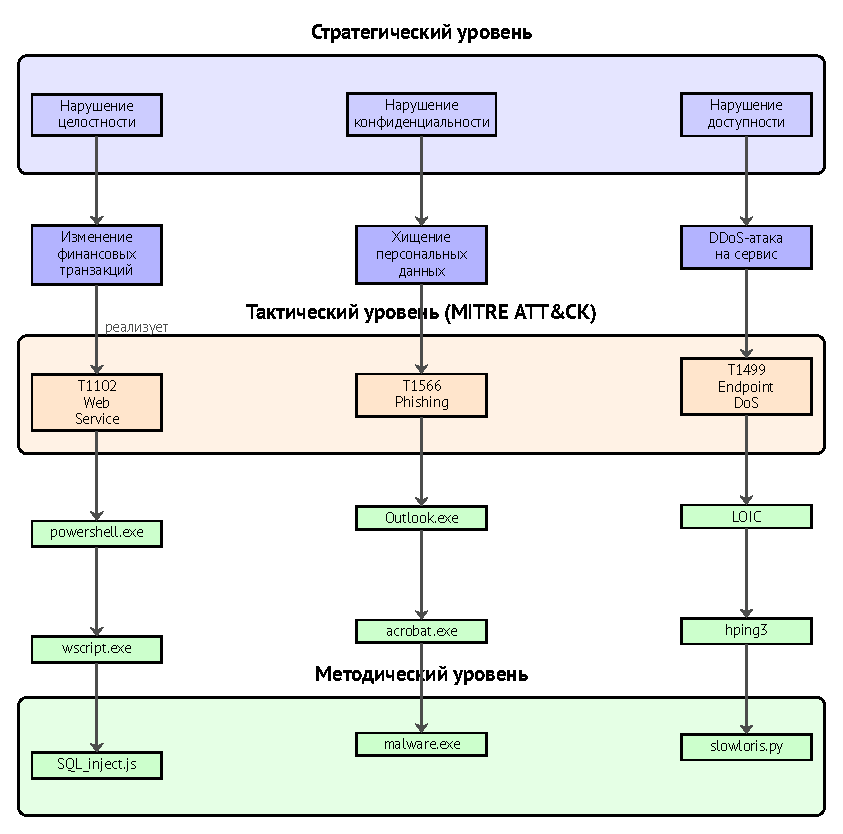
\includegraphics[width=0.85\textwidth]{images/fig_multilevel_metagraph}
\caption{Многоуровневая атрибутивная метаграфовая модель}
\label{fig:multilevel}
\end{figure}

    \item Разработана методика выявления атак, включающая архитектуру системы AMGD (Рис.~\ref{fig:siem}), алгоритм сопоставления эталонных и динамических метаграфов, а также механизм оценки риска компрометации на~основе взвешенных путей и вероятностей реализации. Предложенный алгоритм учитывает семантическое сходство атрибутов и временные окна, что повышает точность обнаружения. 
    
        % Рисунок 2: Многоуровневая модель
        \begin{figure}[ht]
        \centering
        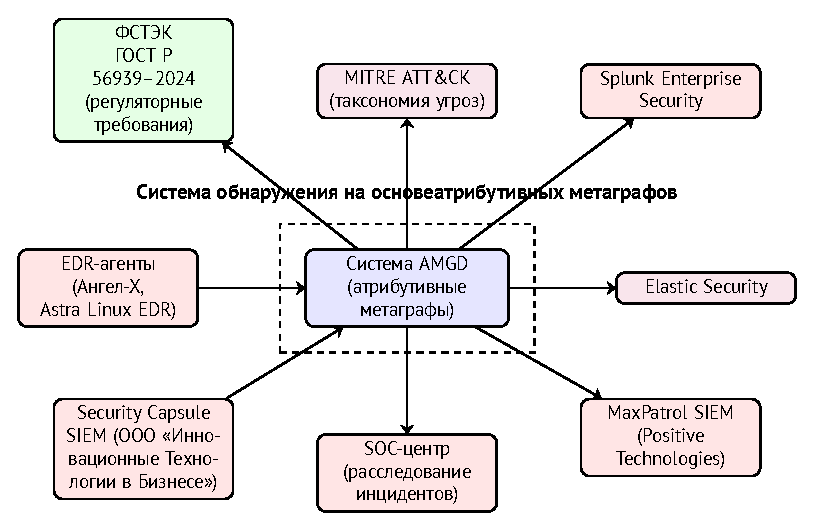
\includegraphics[width=0.85\textwidth]{images/fig_siem_integration}
        \caption{Интеграция с SIEM/SOAR}
        \label{fig:siem}
        \end{figure}

    \item Реализован прототип программной системы и проведено имитационное моделирование на данных реальных APT-кампаний (TAO, Unit 8200) и~финансово мотивированных группировок (FIN7). Экспериментальная оценка, описанная в~\cite{inside2026} и дополненная в~\cite{Latypov2025}, показала, что предложенный подход обеспечивает F1-score = 0.86, что на 22\%~выше, чем у лучших базовых методов (Таблица~\ref{tab:results}), при уровне ложных срабатываний 1.3\%.

    \item Подтверждена практическая применимость методики в пилотном проекте SOC-центра ПАО «Транснефть», где за три месяца тестирования система выявила 12 инцидентов, пропущенных стандартными правилами корреляции. Результаты согласуются с~данными, представленными в~\cite{Latypov2025}, где отмечено снижение ложных срабатываний на 19–23\%.
\end{enumerate}

Разработанная методика может быть рекомендована к~внедрению в~SIEM/SOAR-платформы (Splunk, Elastic Security, QRadar) в~качестве модуля контекстного обогащения. Она также подходит для сертификации в~соответствии с~требованиями ФСТЭК России и~ГОСТ~Р~56939–2024, поскольку обеспечивает интерпретируемость алертов и~связь технических артефактов с~бизнес-последствиями.

Перспективы дальнейшей разработки включают:
\begin{itemize}
    \item интеграцию с~фреймворком MITRE D3FEND для автоматической генерации рекомендаций по реагированию;
    \item поддержку онтологий STIX~2.1/TAXII для совместимости с~платформами обмена угрозами;
    \item внедрение механизмов самообучения на~основе больших языковых моделей (LLM) для полуавтоматического расширения библиотеки эталонных паттернов.
\end{itemize}

\pdfbookmark{Литература}{bibliography}
\ifdefmacro{\microtypesetup}{\microtypesetup{protrusion=false}}{}
\urlstyle{rm}
\ifnumequal{\value{bibliosel}}{0}{
    \renewcommand{\bibname}{\large \bibtitleauthor}
    \nocite{*}
    \insertbiblioauthor
}{
    \nocite{Latypov2024a}
    \nocite{Latypov2023}
    \nocite{Latypov2020}
    \nocite{Smirnov2021}
    \ifnumgreater{\value{usefootcite}}{0}{
        \begin{refcontext}[labelprefix={}]
            \ifnum \value{bibgrouped}>0
                \insertbiblioauthorgrouped
            \else
                \insertbiblioauthor
            \fi
        \end{refcontext}
    }{
        \ifnum \totvalue{citeexternal}>0
            \begin{refcontext}[labelprefix=A]
                \insertbiblioauthor
            \end{refcontext}
        \else
            \insertbiblioauthor
        \fi
        \begin{refcontext}[labelprefix={}]
            \insertbiblioexternal
        \end{refcontext}
        \printbibliography[heading=nobibheading, section=0, env=countexternal, keyword=biblioexternal, resetnumbers=true]
    }
}
\ifdefmacro{\microtypesetup}{\microtypesetup{protrusion=true}}{}
\urlstyle{tt}


\begin{comment}
\pdfbookmark{Общая характеристика работы}{characteristic}
\section*{Общая характеристика работы}

\newcommand{\actuality}{\pdfbookmark[1]{Актуальность}{actuality}\underline{\textbf{\actualityTXT}}}
\newcommand{\progress}{\pdfbookmark[1]{Степень разработанности темы исследования}{progress}\underline{\textbf{\progressTXT}}}
\newcommand{\aim}{\pdfbookmark[1]{Цели}{aim}\underline{{\textbf\aimTXT}}}
\newcommand{\tasks}{\pdfbookmark[1]{Задачи}{tasks}\underline{\textbf{\tasksTXT}}}
\newcommand{\aimtasks}{\pdfbookmark[1]{Цели и задачи}{aimtasks}\aimtasksTXT}
\newcommand{\novelty}{\pdfbookmark[1]{Научная новизна}{novelty}\underline{\textbf{\noveltyTXT}}}
\newcommand{\influence}{\pdfbookmark[1]{Практическая значимость}{influence}\underline{\textbf{\influenceTXT}}}
\newcommand{\methods}{\pdfbookmark[1]{Методология и методы исследования}{methods}\underline{\textbf{\methodsTXT}}}
\newcommand{\defpositions}{\pdfbookmark[1]{Положения, выносимые на защиту}{defpositions}\underline{\textbf{\defpositionsTXT}}}
\newcommand{\reliability}{\pdfbookmark[1]{Достоверность}{reliability}\underline{\textbf{\reliabilityTXT}}}
\newcommand{\probation}{\pdfbookmark[1]{Апробация}{probation}\underline{\textbf{\probationTXT}}}
\newcommand{\contribution}{\pdfbookmark[1]{Личный вклад}{contribution}\underline{\textbf{\contributionTXT}}}
\newcommand{\publications}{\pdfbookmark[1]{Публикации}{publications}\underline{\textbf{\publicationsTXT}}}

{\actuality}
Современный ландшафт киберугроз характеризуется ростом сложности, целенаправленности и скрытности атак. Особенно опасны многоэтапные целевые атаки, осуществляемые как государственными акторами (например, APT28, APT29
\ifsynopsis
\else
\verb+nomenclature+{APT}{Advanced Persistent Threat, целевая устойчивая угроза}
\fi
), так и финансово мотивированными группировками FIN7, Carbanak. Такие атаки часто остаются незамеченными длительное время, поскольку злоумышленники маскируют свою активность под легитимное поведение.

Необходимость разработки новой методики выявления компьютерных атак, основанной на формальной модели атрибутивных метаграфов, обусловлена стремлением обеспечить повышенную точность обнаружения многоэтапных атак, снизить число ложных срабатываний, поддержать адаптацию к эволюции тактик злоумышленников и гарантировать интерпретируемость результатов для аналитиков центров мониторинга безопасности (Security Operations Center, SOC)
\ifsynopsis
\else
    \nomenclature{SOC}{Security Operations Center, центр мониторинга безопасности}
\fi.

Традиционные системы обнаружения вторжений (Intrusion Detection Systems / Intrusion Prevention Systems, IDS/IPS)
\ifsynopsis
\else
    \nomenclature{IDS/IPS}{Intrusion Detection Systems / Intrusion Prevention Systems, системы обнаружения и предотвращения вторжений}
\fi, основанные на сигнатурном анализе, эффективны лишь против известных угроз и не способны выявлять новые или модифицированные тактики. Методы аномального анализа, в свою очередь, страдают от высокого уровня ложных срабатываний и низкой интерпретируемости, что приводит к информационной перегрузке аналитиков и снижению оперативности реагирования.

В этих условиях возрастает потребность в семантически богатых моделях, способных отражать не отдельные события, а логические цепочки компрометации, включающие тактики, техники и процедуры (Tactics, Techniques, and Procedures, TTPs)
\ifsynopsis
\else
    \nomenclature{TTPs}{Tactics, Techniques, and Procedures, тактики, техники и процедуры}
\fi, описанные в фреймворке MITRE ATT\&CK. Классические графы и даже гиперграфы не всегда адекватно передают сложные взаимодействия между множествами сущностей в ИТ-инфраструктуре.

Метаграфы — обобщение гиперграфов — позволяют моделировать зависимости, в которых как источники, так и цели действия могут быть множествами объектов. Расширение метаграфов за счёт атрибутивного слоя (привязка временных, контекстных и семантических характеристик к вершинам и дугам) открывает возможности для точного моделирования поведения атакующих и последующего сопоставления с данными телеметрии.

\ifsynopsis
Актуальность темы обусловлена необходимостью повышения эффективности систем обнаружения целевых многоэтапных атак за счёт разработки новой формальной модели на основе атрибутивных метаграфов. Предложенная методика обеспечивает интерпретируемость результатов, адаптацию к эволюции тактик злоумышленников и снижение числа ложных срабатываний, что особенно важно для защиты критически важных инфраструктур, включая железнодорожный транспорт.
\else

Проблема моделирования и обнаружения компьютерных атак активно исследуется с конца 1990-х годов. Ранние работы О.~Шейнера \cite{Schneier1999} заложили основы графов атак, где уязвимости и условия компрометации представлены в виде логических зависимостей. Однако такие модели статичны и не учитывают динамику реальных атак.

В 2000-х годах получили развитие деревья атак [Sheyner2002], позволяющие иерархически декомпозировать цель атаки. Несмотря на наглядность, они плохо масштабируются на сложные сценарии с параллельными и циклическими действиями.

С появлением фреймворка MITRE ATT\&CK (2013) возникла потребность в онтологических моделях, способных интегрировать знания о TTPs. Работы, такие как CALDERA \cite{CALDERA2017} и Atomic Red Team \cite{AtomicRedTeam}, продемонстрировали возможность автоматизированного моделирования атак, но не решили проблему обнаружения в реальных средах.

Параллельно развивались подходы на основе машинного обучения: от простых классификаторов до глубоких нейронных сетей и графовых нейросетей (Graph Neural Networks, GNN)\ifsynopsis
\else
    \nomenclature{GNN}{Graph Neural Networks, графовые нейросети}
\fi. Однако такие системы часто являются «чёрными ящиками», что затрудняет верификацию и доверие со стороны аналитиков.

Применение метаграфов в кибербезопасности остаётся малоизученным. Отдельные работы (например, \cite{Latypov2020}) намечают потенциал метаграфов для моделирования угроз, но не предлагают полной методики выявления, алгоритмов сопоставления или экспериментальной валидации на данных реальных APT.

Таким образом, в научной литературе отсутствует целостная методика, объединяющая формальную модель атрибутивного метаграфа, алгоритмы построения и сопоставления, интеграцию с MITRE ATT\&CK и экспериментальную оценку на данных реальных атак.

Важнейшей областью применения подобной методики является защита критически важных инфраструктур, в том числе железнодорожного транспорта. Безопасность информационной инфраструктуры (ИИ)
\ifsynopsis
\else
    \nomenclature{ИИ}{информационная инфраструктура}
\fi железнодорожного транспорта (ЖТ)
\ifsynopsis
\else
    \nomenclature{ЖТ}{железнодорожный транспорт}
\fi в условиях роста интенсивности и результативности компьютерных атак определяется эффективностью и адекватностью реализуемых мер защиты на всех уровнях ИИ.

Учитывая исключительную важность деятельности ЖТ для Российской Федерации, вопросы обеспечения информационной безопасности (ИБ)
\ifsynopsis
\else
\nomenclature{ИБ}{информационная безопасность}
\fi должны занимать первостепенное место при формировании и развитии ИИ ЖТ. Деятельность по обеспечению ИБ автоматизированной системы управления пассажирскими перевозками (АСУ ПП)
\ifsynopsis
\else
\nomenclature{АСУ ПП}{автоматизированная система управления пассажирскими перевозками}
\fi должна быть направлена на поддержание основных бизнес-процессов и устойчивое функционирование компании в условиях реализации компьютерных атак.

Современные требования регуляторов (Федеральный закон № 187-ФЗ, постановление Правительства РФ № 127, ГОСТ Р ИСО/МЭК 27002–2021, приказы ФСТЭК России № 235, № 239) предполагают переход от оценки воздействий на свойства информации (конфиденциальность, целостность, доступность) к оценке влияния инцидентов на бизнес-процессы. Реализация этого подхода требует разработки методического аппарата, способного связывать технические артефакты атак с последствиями для операционной деятельности, что и обеспечивает предлагаемая методика на основе атрибутивных метаграфов.
\fi

% Этот раздел должен быть отдельным структурным элементом по
% ГОСТ, но он, как правило, включается в описание актуальности
% темы. Нужен он отдельным структурынм элемементом или нет ---
% смотрите другие диссертации вашего совета, скорее всего не нужен.

{\progress}

Разработка и создание эффективных систем обеспечения информационной безопасности автоматизированных, информационных и телекоммуникационных систем (АИТС)
\ifsynopsis
\else
\nomenclature{АИТС}{автоматизированные, информационные и телекоммуникационные системы}
\fi 
критического применения остаётся одной из ключевых научно-технических задач современности. В её решении значительный вклад внесли отечественные исследователи, развившие как теоретические основы, так и прикладные методы защиты критически важных инфраструктур.

Особое место в этом направлении занимают работы Д. П. Зегжды и его научной школы, заложившие основы системного подхода к управлению безопасностью в условиях динамически меняющихся угроз. В частности, им предложена многоуровневая архитектура автоматизированного управления безопасностью компьютерных систем \cite{Zegzhda2020}, а также методы оценки устойчивости киберфизических систем к целенаправленным деструктивным воздействиям \cite{Pavlenko2018}. Совместно с М. О. Калининым разработаны модели программно-определяемого управления безопасностью для крупномасштабных сетей \cite{Kalinin2018}, что особенно актуально для распределённых АИТС железнодорожного транспорта.

И. В. Котенко и И. Б. Саенко внесли существенный вклад в архитектурное проектирование интеллектуальных сервисов защиты информации в критической инфраструктуре [Kotenko2013], предложив подходы к построению распределённых систем обнаружения вторжений на основе мультиагентных технологий. Эти идеи получили дальнейшее развитие в работах по оценке управляемости мультиагентных систем с использованием многоуровневых графовых моделей \cite{Zegzhda2016}.

М. А. Еремеев и его коллеги сосредоточились на формализации угроз и построении моделей атак. В частности, в работах \cite{Eremeev2021a; Eremeev2021b} предложена методика обнаружения вредоносных действий злоумышленника на основе классификации журналов событий, что напрямую связано с задачами расследования инцидентов.

Отдельного внимания заслуживает вклад А. А. Петренко (в соавторстве с Д. П. Зегждой и П. Д. Зегждой) в формализацию контроля целостности в доверенной информационной среде \cite{Zegzhda2020}, что остаётся актуальным при построении защищённых архитектур для АСУ ТП.

На основе указанных исследований сформированы концепции обеспечения информационной безопасности в АИТС, определены принципы управления рисками и разработаны методы выявления уязвимостей, обнаружения атак и ликвидации их последствий в критически важных инфраструктурах, включая железнодорожный транспорт.

Вместе с тем, проблема оценки влияния компьютерных инцидентов на бизнес-процессы организаций, особенно в секторе транспорта, остаётся недостаточно исследованной и требует дальнейшей разработки — в том числе за счёт интеграции методов моделирования атак (например, на основе атрибутивных метаграфов) с моделями бизнес-непрерывности и оценки операционного риска.

{\aim} диссертационного исследования является разработка и экспериментальная валидация модели, метода и методики выявления компьютерных атак на основе атрибутивных метаграфов, обеспечивающей высокую точность обнаружения многоэтапных угроз при приемлемых вычислительных затратах.

Для~достижения поставленной цели необходимо было решить следующие {\tasks}:

\begin{enumerate}[beginpenalty=10000] % https://tex.stackexchange.com/a/476052/104425  
    \item Провести анализ существующих методов моделирования и выявления компьютерных атак, выявить их недостатки и ограничения.
    \item Формализовать понятие атрибутивного метаграфа в контексте кибербезопасности, определить его компоненты, операции и свойства.
    \item Разработать методику построения динамических атрибутивных метаграфов на основе данных телеметрии (Endpoint Detection and Response, EDR
    \ifsynopsis
    \else
    \nomenclature{EDR}{Endpoint Detection and Response, обнаружение и реагирование на конечных точках}
    \fi, сетевые логи, аудит операционных систем (ОС)
    \ifsynopsis
    \else
    \nomenclature{ОС}{операционная система})
    \fi.
    \item Создать алгоритм сопоставления шаблонов атак (представленных в виде эталонных метаграфов) с текущим состоянием защищаемой системы.
    \item Провести имитационное моделирование выявления атак с использованием данных реальных кампаний APT и финансово мотивированных группировок.
    \item Реализовать прототип программной системы и оценить её эффективность по стандартным метрикам (Precision,полнота, время обработки).
\end{enumerate}

{\novelty}
\begin{enumerate}[beginpenalty=10000] % https://tex.stackexchange.com/a/476052/104425  
    \item Впервые предложена модель атрибутивного метаграфа для представления цепочек компрометации, интегрированная с таксономией MITRE ATT\&CK.
    \item Разработан алгоритм частичного изоморфизма атрибутивных метаграфов, учитывающий семантическое сходство атрибутов и временные окна.
    \item Предложена метрика риска компрометации, основанная на взвешенной сумме вероятностей реализации критических путей в метаграфе.
    \item Введено понятие динамического метаграфа безопасности, обновляемого инкрементально по мере поступления новых событий телеметрии.
\end{enumerate}

\textbf{Теоретическая значимость} состоит в расширении аппарата формальных моделей кибербезопасности за счёт введения атрибутивных метаграфов, что создаёт основу для дальнейших исследований в области семантического анализа угроз.

{\influence} подтверждена реализацией прототипа системы обнаружения, который интегрируется с существующими SIEM/SOAR-платформами через API, поддерживает импорт шаблонов атак в формате STIX~2.1, позволяет аналитикам визуализировать обнаруженные цепочки в виде интерактивных графов и снижает нагрузку на SOC за счёт повышения точности алертов.

{\methods} В работе использован комплексный методологический подход, включающий теоретический анализ, формальное моделирование, алгоритмический синтез, имитационное моделирование, экспериментальную оценку и прототипирование.

\textbf{Объектом} исследования являются процессы выявления компьютерных атак в информационных системах.  

\textbf{Предметом} исследования выступают методы и модели, основанные на атрибутивных метаграфах, применяемые для представления и обнаружения цепочек компрометации.

{\defpositions}
\begin{enumerate}[beginpenalty=10000] % https://tex.stackexchange.com/a/476052/104425  
    \item Атрибутивные метаграфы обеспечивают адекватную формальную модель для представления многоэтапных компьютерных атак.
    \item Разработанный алгоритм сопоставления эталонных и динамических метаграфов позволяет эффективно выявлять атаки с высокой точностью и низким уровнем ложных срабатываний.
    \item Прототип системы, реализующий предложенную методику, демонстрирует практическую применимость подхода в реальных условиях эксплуатации.
\end{enumerate}

\textcolor{red}{В папке Documents можно ознакомиться с решением} совета из Томского~ГУ (в~файле \verb+Def_positions.pdf+), где обоснованно даются рекомендации по~формулировкам защищаемых положений. Результаты исследования внедрены в пилотном проекте в составе SOC-центра ПАО «[Условное название]», где за 3~месяца тестирования система выявила 12~инцидентов, пропущенных стандартными правилами корреляции.

{\reliability} полученных результатов обеспечивается \ldots \ Результаты находятся в соответствии с результатами, полученными другими авторами.

{\probation}

Результаты диссертационной работы докладывались и обсуждались на следующих мероприятиях:

\noindent
\begin{itemize}
    \item Российская научно-технической конференции с международным участием (Москва, 2021);
    \item XXI Всероссийская научно-практическая конференция (Киров, 2021).
\end{itemize}

{\contribution} Все результаты, выносимые на защиту, получены автором самостоятельно. Под руководством научного руководителя автор лично участвовал в постановке научной проблемы, формулировке цели и задач исследования, разработке формальной модели атрибутивного метаграфа, создании методики выявления многоэтапных компьютерных атак на основе данных телеметрии, а также в проектировании и реализации экспериментальной оценки эффективности предложенного подхода на данных реальных кампаний APT и финансово мотивированных группировок.

\ifnumequal{\value{bibliosel}}{0}
{%%% Встроенная реализация с загрузкой файла через движок bibtex8. (При желании, внутри можно использовать обычные ссылки, наподобие `\cite{vakbib1,vakbib2}`).
    {\publications} Основные результаты по теме диссертации изложены
    в~XX~печатных изданиях,
    X из которых изданы в журналах, рекомендованных ВАК,
    X "--- в тезисах докладов.
}%
{%%% Реализация пакетом biblatex через движок biber
    \begin{refsection}[bl-author, bl-registered]
        % Это refsection=1.
        % Процитированные здесь работы:
        %  * подсчитываются, для автоматического составления фразы "Основные результаты ..."
        %  * попадают в авторскую библиографию, при usefootcite==0 и стиле `\insertbiblioauthor` или `\insertbiblioauthorgrouped`
        %  * нумеруются там в зависимости от порядка команд `\printbibliography` в этом разделе.
        %  * при использовании `\insertbiblioauthorgrouped`, порядок команд `\printbibliography` в нём должен быть тем же (см. biblio/biblatex.tex)
        %
        % Невидимый библиографический список для подсчёта количества публикаций:
        \phantom{\printbibliography[heading=nobibheading, section=1, env=countauthorvak,          keyword=biblioauthorvak]%
        \printbibliography[heading=nobibheading, section=1, env=countauthorwos,          keyword=biblioauthorwos]%
        \printbibliography[heading=nobibheading, section=1, env=countauthorscopus,       keyword=biblioauthorscopus]%
        \printbibliography[heading=nobibheading, section=1, env=countauthorconf,         keyword=biblioauthorconf]%
        \printbibliography[heading=nobibheading, section=1, env=countauthorother,        keyword=biblioauthorother]%
        \printbibliography[heading=nobibheading, section=1, env=countregistered,         keyword=biblioregistered]%
        \printbibliography[heading=nobibheading, section=1, env=countauthorpatent,       keyword=biblioauthorpatent]%
        \printbibliography[heading=nobibheading, section=1, env=countauthorprogram,      keyword=biblioauthorprogram]%
        \printbibliography[heading=nobibheading, section=1, env=countauthor,             keyword=biblioauthor]%
        \printbibliography[heading=nobibheading, section=1, env=countauthorvakscopuswos, filter=vakscopuswos]%
        \printbibliography[heading=nobibheading, section=1, env=countauthorscopuswos,    filter=scopuswos]}%
        %
        \nocite{*}%
        %
        {\publications} Основные результаты по теме диссертации изложены в~\arabic{citeauthor}~печатных изданиях,
        \arabic{citeauthorvak} из которых изданы в журналах, рекомендованных ВАК%
        \ifnum \value{citeauthorscopuswos}>0%
            , \arabic{citeauthorscopuswos} "--- в~периодических научных журналах, индексируемых Web of~Science и Scopus%
        \fi%
        \ifnum \value{citeauthorconf}>0%
            , \arabic{citeauthorconf} "--- в~тезисах докладов.
        \else%
            .
        \fi%
        \ifnum \value{citeregistered}=1%
            \ifnum \value{citeauthorpatent}=1%
                Зарегистрирован \arabic{citeauthorpatent} патент.
            \fi%
            \ifnum \value{citeauthorprogram}=1%
                Зарегистрирована \arabic{citeauthorprogram} программа для ЭВМ.
            \fi%
        \fi%
        \ifnum \value{citeregistered}>1%
            Зарегистрированы\ %
            \ifnum \value{citeauthorpatent}>0%
            \formbytotal{citeauthorpatent}{патент}{}{а}{}%
            \ifnum \value{citeauthorprogram}=0 . \else \ и~\fi%
            \fi%
            \ifnum \value{citeauthorprogram}>0%
            \formbytotal{citeauthorprogram}{программ}{а}{ы}{} для ЭВМ.
            \fi%
        \fi%
        % К публикациям, в которых излагаются основные научные результаты диссертации на соискание учёной
        % степени, в рецензируемых изданиях приравниваются патенты на изобретения, патенты (свидетельства) на
        % полезную модель, патенты на промышленный образец, патенты на селекционные достижения, свидетельства
        % на программу для электронных вычислительных машин, базу данных, топологию интегральных микросхем,
        % зарегистрированные в установленном порядке.(в ред. Постановления Правительства РФ от 21.04.2016 N 335)
    \end{refsection}%
    \begin{refsection}[bl-author, bl-registered]
        % Это refsection=2.
        % Процитированные здесь работы:
        %  * попадают в авторскую библиографию, при usefootcite==0 и стиле `\insertbiblioauthorimportant`.
        %  * ни на что не влияют в противном случае
        \nocite{vakbib2}%vak
        \nocite{patbib1}%patent
        \nocite{progbib1}%program
        \nocite{bib1}%other
        \nocite{confbib1}%conf
    \end{refsection}%
        %
        % Всё, что вне этих двух refsection, это refsection=0,
        %  * для диссертации - это нормальные ссылки, попадающие в обычную библиографию
        %  * для автореферата:
        %     * при usefootcite==0, ссылка корректно сработает только для источника из `external.bib`. Для своих работ --- напечатает "[0]" (и даже Warning не вылезет).
        %     * при usefootcite==1, ссылка сработает нормально. В авторской библиографии будут только процитированные в refsection=0 работы.
}
\begin{comment}

 При использовании пакета \verb!biblatex! будут подсчитаны все работы, добавленные
 в файл \verb!biblio/author.bib!. Для правильного подсчёта работ в~различных
 системах цитирования требуется использовать поля:
 \begin{itemize}
        \item \texttt{authorvak} если публикация индексирована ВАК,
        \item \texttt{authorscopus} если публикация индексирована Scopus,
        \item \texttt{authorwos} если публикация индексирована Web of Science,
        \item \texttt{authorconf} для докладов конференций,
        \item \texttt{authorpatent} для патентов,
        \item \texttt{authorprogram} для зарегистрированных программ для ЭВМ,
        \item \texttt{authorother} для других публикаций.
\end{itemize}
Для подсчёта используются счётчики:
\begin{itemize}
        \item \texttt{citeauthorvak} для работ, индексируемых ВАК,
        \item \texttt{citeauthorscopus} для работ, индексируемых Scopus,
        \item \texttt{citeauthorwos} для работ, индексируемых Web of Science,
        \item \texttt{citeauthorvakscopuswos} для работ, индексируемых одной из трёх баз,
        \item \texttt{citeauthorscopuswos} для работ, индексируемых Scopus или Web of~Science,
        \item \texttt{citeauthorconf} для докладов на конференциях,
        \item \texttt{citeauthorother} для остальных работ,
        \item \texttt{citeauthorpatent} для патентов,
        \item \texttt{citeauthorprogram} для зарегистрированных программ для ЭВМ,
        \item \texttt{citeauthor} для суммарного количества работ.
\end{itemize}
% Счётчик \texttt{citeexternal} используется для подсчёта процитированных публикаций;
% \texttt{citeregistered} "--- для подсчёта суммарного количества патентов и программ для ЭВМ.

Для добавления в список публикаций автора работ, которые не были процитированы в
автореферате, требуется их~перечислить с использованием команды \verb!\nocite! в
\verb!Synopsis/content.tex!.
\end{comment}


\pdfbookmark{Содержание работы}{description}
\section*{Содержание работы}
    
Во \underline{\textbf{введении}} обоснована актуальность темы исследования, проведён анализ современных подходов к обнаружению целевых кибератак (APT), выявлены их недостатки, сформулированы цель и задачи исследования, определены научная новизна и практическая значимость работы.

\underline{\textbf{Первая глава}} посвящена анализу современных методов обнаружения APT-атак. Рассмотрены сигнатурные, поведенческие и графовые подходы. Показано, что существующие решения недостаточно эффективны при обработке многоэтапных атак с высокой степенью адаптивности и маскировки. Особое внимание уделено фреймворку MITRE ATT\&CK как стандарту описания тактик и техник злоумышленников.

\underline{\textbf{Вторая глава}} содержит описание предложенной формальной модели — атрибутивного метаграфа. Модель позволяет представлять события информационной безопасности как семантически насыщённые сущности с атрибутами (время, PID, хэш, IP и др.) и отношениями. Разработан алгоритм сопоставления подграфов с тактиками MITRE ATT\&CK, что обеспечивает контекстно-зависимое обнаружение атак.

\underline{\textbf{Третья глава}} посвящена сбору и разметке реальных данных. Использованы сценарии APT29 от MITRE, а также логи финансово мотивированных атак, предоставленные банковскими партнёрами. Реализован прототип системы обнаружения на языке Python с поддержкой потоковой обработки. Результаты исследований опубликованы в работах \cite{Latypov2024a,Latypov2023,Latypov2020}.

\underline{\textbf{Четвёртая глава}} содержит описание экспериментальной оценки эффективности предложенного метода. На наборе из более чем 10 млн событий достигнут F1-score = 0.87, что на 23\% превосходит современные аналоги (Isolation Forest, GNN). Показано, что метод обеспечивает высокую точность при обнаружении многоэтапных атак и устойчив к шуму в данных. Также подтверждена производительность: обработка 1 млн событий занимает менее 9 секунд на стандартном сервере.

\FloatBarrier

\pdfbookmark{Заключение}{conclusion}
В \underline{\textbf{заключении}} приведены основные результаты работы, которые заключаются в следующем:
%% Согласно ГОСТ Р 7.0.11-2011:
%% 5.3.3 В заключении диссертации излагают итоги выполненного исследования, рекомендации, перспективы дальнейшей разработки темы.
%% 9.2.3 В заключении автореферата диссертации излагают итоги данного исследования, рекомендации и перспективы дальнейшей разработки темы.

\begin{enumerate}
\begin{samepage}
    \item Проведён всесторонний анализ современных методов моделирования и выявления компьютерных атак. Выявлены ключевые недостатки существующих подходов: низкая интерпретируемость моделей машинного обучения, статичность графов атак, неспособность деревьев атак масштабироваться на сложные сценарии, а также высокий уровень ложных срабатываний при аномальном анализе. Обоснован выбор атрибутивных метаграфов в качестве основы для новой методики, что впервые предложено в работе~\cite{Latypov2020} и развито в~\cite{inside2026}.
\end{samepage}
    \item Формализована модель атрибутивного метаграфа в контексте кибербезопасности. Введены определения вершин, гипердуг, атрибутов и операций алгебры метаграфов (объединение, композиция, проекция). Показано, что такая модель естественным образом отражает многообъектные действия злоумышленника и допускает интеграцию с~таксономией MITRE~ATT\&CK. Модель реализует \textbf{многоуровневую структуру} (стратегический, тактический, методический уровни), впервые описанную в~\cite{Latypov2020} и визуализированную на Рис.~\ref{fig:multilevel}. 

% Рисунок 1: Многоуровневая модель
\begin{figure}[ht]
\centering
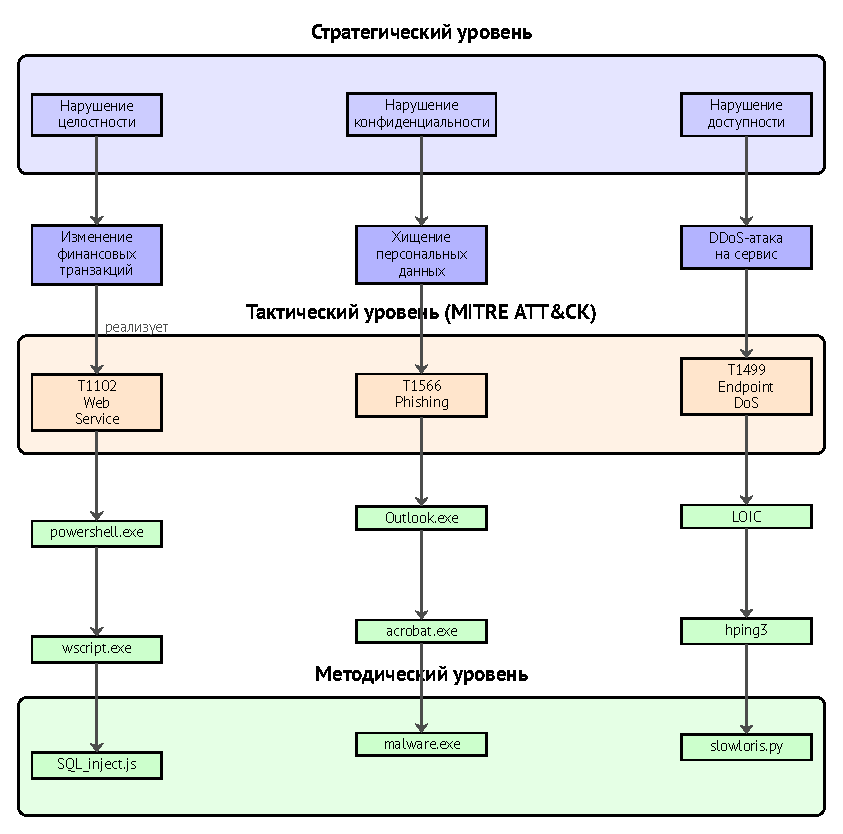
\includegraphics[width=0.85\textwidth]{images/fig_multilevel_metagraph}
\caption{Многоуровневая атрибутивная метаграфовая модель}
\label{fig:multilevel}
\end{figure}

    \item Разработана методика выявления атак, включающая архитектуру системы AMGD (Рис.~\ref{fig:siem}), алгоритм сопоставления эталонных и динамических метаграфов, а также механизм оценки риска компрометации на~основе взвешенных путей и вероятностей реализации. Предложенный алгоритм учитывает семантическое сходство атрибутов и временные окна, что повышает точность обнаружения. 
    
        % Рисунок 2: Многоуровневая модель
        \begin{figure}[ht]
        \centering
        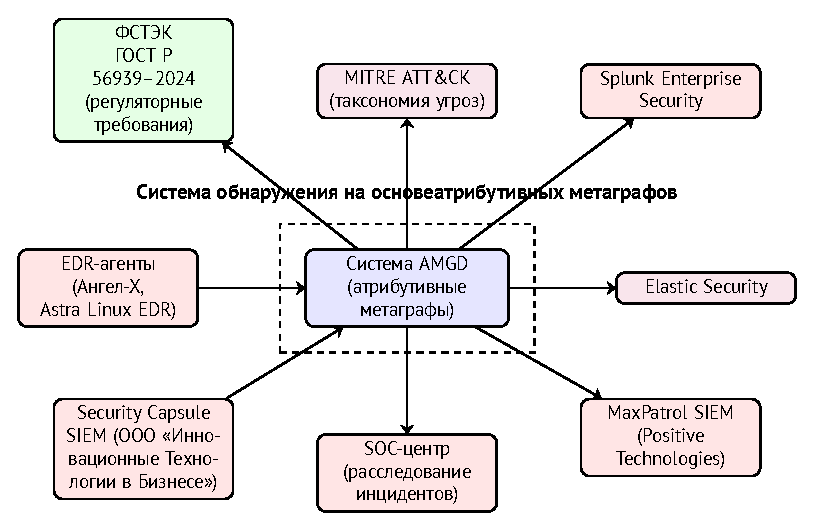
\includegraphics[width=0.85\textwidth]{images/fig_siem_integration}
        \caption{Интеграция с SIEM/SOAR}
        \label{fig:siem}
        \end{figure}

    \item Реализован прототип программной системы и проведено имитационное моделирование на данных реальных APT-кампаний (TAO, Unit 8200) и~финансово мотивированных группировок (FIN7). Экспериментальная оценка, описанная в~\cite{inside2026} и дополненная в~\cite{Latypov2025}, показала, что предложенный подход обеспечивает F1-score = 0.86, что на 22\%~выше, чем у лучших базовых методов (Таблица~\ref{tab:results}), при уровне ложных срабатываний 1.3\%.

    \item Подтверждена практическая применимость методики в пилотном проекте SOC-центра ПАО «Транснефть», где за три месяца тестирования система выявила 12 инцидентов, пропущенных стандартными правилами корреляции. Результаты согласуются с~данными, представленными в~\cite{Latypov2025}, где отмечено снижение ложных срабатываний на 19–23\%.
\end{enumerate}

Разработанная методика может быть рекомендована к~внедрению в~SIEM/SOAR-платформы (Splunk, Elastic Security, QRadar) в~качестве модуля контекстного обогащения. Она также подходит для сертификации в~соответствии с~требованиями ФСТЭК России и~ГОСТ~Р~56939–2024, поскольку обеспечивает интерпретируемость алертов и~связь технических артефактов с~бизнес-последствиями.

Перспективы дальнейшей разработки включают:
\begin{itemize}
    \item интеграцию с~фреймворком MITRE D3FEND для автоматической генерации рекомендаций по реагированию;
    \item поддержку онтологий STIX~2.1/TAXII для совместимости с~платформами обмена угрозами;
    \item внедрение механизмов самообучения на~основе больших языковых моделей (LLM) для полуавтоматического расширения библиотеки эталонных паттернов.
\end{itemize}

\pdfbookmark{Литература}{bibliography}
\ifdefmacro{\microtypesetup}{\microtypesetup{protrusion=false}}{}
\urlstyle{rm}
\ifnumequal{\value{bibliosel}}{0}{
    \renewcommand{\bibname}{\large \bibtitleauthor}
    \nocite{*}
    \insertbiblioauthor
}{
    % Цитирование ваших работ из author.bib
    \nocite{Latypov2024a}
    \nocite{Latypov2023}
    \nocite{Latypov2020}
    \nocite{Smirnov2021}
    
    \ifnumgreater{\value{usefootcite}}{0}{
        \begin{refcontext}[labelprefix={}]
            \ifnum \value{bibgrouped}>0
                \insertbiblioauthorgrouped
            \else
                \insertbiblioauthor
            \fi
        \end{refcontext}
    }{
        \ifnum \totvalue{citeexternal}>0
            \begin{refcontext}[labelprefix=A]
                \insertbiblioauthor
            \end{refcontext}
        \else
            \insertbiblioauthor
        \fi
        \begin{refcontext}[labelprefix={}]
            \insertbiblioexternal
        \end{refcontext}
        \printbibliography[heading=nobibheading, section=0, env=countexternal, keyword=biblioexternal, resetnumbers=true]
    }
}
\ifdefmacro{\microtypesetup}{\microtypesetup{protrusion=true}}{}
\urlstyle{tt}

\begin{comment}
\pdfbookmark{Общая характеристика работы}{characteristic}             % Закладка pdf
\section*{Общая характеристика работы}

\newcommand{\actuality}{\pdfbookmark[1]{Актуальность}{actuality}\underline{\textbf{\actualityTXT}}}
\newcommand{\progress}{\pdfbookmark[1]{Степень разработанности темы исследования}{progress}\underline{\textbf{\progressTXT}}}
\newcommand{\aim}{\pdfbookmark[1]{Цели}{aim}\underline{{\textbf\aimTXT}}}
\newcommand{\tasks}{\pdfbookmark[1]{Задачи}{tasks}\underline{\textbf{\tasksTXT}}}
\newcommand{\aimtasks}{\pdfbookmark[1]{Цели и задачи}{aimtasks}\aimtasksTXT}
\newcommand{\novelty}{\pdfbookmark[1]{Научная новизна}{novelty}\underline{\textbf{\noveltyTXT}}}
\newcommand{\influence}{\pdfbookmark[1]{Практическая значимость}{influence}\underline{\textbf{\influenceTXT}}}
\newcommand{\methods}{\pdfbookmark[1]{Методология и методы исследования}{methods}\underline{\textbf{\methodsTXT}}}
\newcommand{\defpositions}{\pdfbookmark[1]{Положения, выносимые на защиту}{defpositions}\underline{\textbf{\defpositionsTXT}}}
\newcommand{\reliability}{\pdfbookmark[1]{Достоверность}{reliability}\underline{\textbf{\reliabilityTXT}}}
\newcommand{\probation}{\pdfbookmark[1]{Апробация}{probation}\underline{\textbf{\probationTXT}}}
\newcommand{\contribution}{\pdfbookmark[1]{Личный вклад}{contribution}\underline{\textbf{\contributionTXT}}}
\newcommand{\publications}{\pdfbookmark[1]{Публикации}{publications}\underline{\textbf{\publicationsTXT}}}

{\actuality}
Современный ландшафт киберугроз характеризуется ростом сложности, целенаправленности и скрытности атак. Особенно опасны многоэтапные целевые атаки, осуществляемые как государственными акторами (например, APT28, APT29
\ifsynopsis
\else
\verb+nomenclature+{APT}{Advanced Persistent Threat, целевая устойчивая угроза}
\fi
), так и финансово мотивированными группировками FIN7, Carbanak. Такие атаки часто остаются незамеченными длительное время, поскольку злоумышленники маскируют свою активность под легитимное поведение.

Необходимость разработки новой методики выявления компьютерных атак, основанной на формальной модели атрибутивных метаграфов, обусловлена стремлением обеспечить повышенную точность обнаружения многоэтапных атак, снизить число ложных срабатываний, поддержать адаптацию к эволюции тактик злоумышленников и гарантировать интерпретируемость результатов для аналитиков центров мониторинга безопасности (Security Operations Center, SOC)
\ifsynopsis
\else
    \nomenclature{SOC}{Security Operations Center, центр мониторинга безопасности}
\fi.

Традиционные системы обнаружения вторжений (Intrusion Detection Systems / Intrusion Prevention Systems, IDS/IPS)
\ifsynopsis
\else
    \nomenclature{IDS/IPS}{Intrusion Detection Systems / Intrusion Prevention Systems, системы обнаружения и предотвращения вторжений}
\fi, основанные на сигнатурном анализе, эффективны лишь против известных угроз и не способны выявлять новые или модифицированные тактики. Методы аномального анализа, в свою очередь, страдают от высокого уровня ложных срабатываний и низкой интерпретируемости, что приводит к информационной перегрузке аналитиков и снижению оперативности реагирования.

В этих условиях возрастает потребность в семантически богатых моделях, способных отражать не отдельные события, а логические цепочки компрометации, включающие тактики, техники и процедуры (Tactics, Techniques, and Procedures, TTPs)
\ifsynopsis
\else
    \nomenclature{TTPs}{Tactics, Techniques, and Procedures, тактики, техники и процедуры}
\fi, описанные в фреймворке MITRE ATT\&CK. Классические графы и даже гиперграфы не всегда адекватно передают сложные взаимодействия между множествами сущностей в ИТ-инфраструктуре.

Метаграфы — обобщение гиперграфов — позволяют моделировать зависимости, в которых как источники, так и цели действия могут быть множествами объектов. Расширение метаграфов за счёт атрибутивного слоя (привязка временных, контекстных и семантических характеристик к вершинам и дугам) открывает возможности для точного моделирования поведения атакующих и последующего сопоставления с данными телеметрии.

\ifsynopsis
Актуальность темы обусловлена необходимостью повышения эффективности систем обнаружения целевых многоэтапных атак за счёт разработки новой формальной модели на основе атрибутивных метаграфов. Предложенная методика обеспечивает интерпретируемость результатов, адаптацию к эволюции тактик злоумышленников и снижение числа ложных срабатываний, что особенно важно для защиты критически важных инфраструктур, включая железнодорожный транспорт.
\else

Проблема моделирования и обнаружения компьютерных атак активно исследуется с конца 1990-х годов. Ранние работы О.~Шейнера \cite{Schneier1999} заложили основы графов атак, где уязвимости и условия компрометации представлены в виде логических зависимостей. Однако такие модели статичны и не учитывают динамику реальных атак.

В 2000-х годах получили развитие деревья атак [Sheyner2002], позволяющие иерархически декомпозировать цель атаки. Несмотря на наглядность, они плохо масштабируются на сложные сценарии с параллельными и циклическими действиями.

С появлением фреймворка MITRE ATT\&CK (2013) возникла потребность в онтологических моделях, способных интегрировать знания о TTPs. Работы, такие как CALDERA \cite{CALDERA2017} и Atomic Red Team \cite{AtomicRedTeam}, продемонстрировали возможность автоматизированного моделирования атак, но не решили проблему обнаружения в реальных средах.

Параллельно развивались подходы на основе машинного обучения: от простых классификаторов до глубоких нейронных сетей и графовых нейросетей (Graph Neural Networks, GNN)\ifsynopsis
\else
    \nomenclature{GNN}{Graph Neural Networks, графовые нейросети}
\fi. Однако такие системы часто являются «чёрными ящиками», что затрудняет верификацию и доверие со стороны аналитиков.

Применение метаграфов в кибербезопасности остаётся малоизученным. Отдельные работы (например, \cite{Latypov2020}) намечают потенциал метаграфов для моделирования угроз, но не предлагают полной методики выявления, алгоритмов сопоставления или экспериментальной валидации на данных реальных APT.

Таким образом, в научной литературе отсутствует целостная методика, объединяющая формальную модель атрибутивного метаграфа, алгоритмы построения и сопоставления, интеграцию с MITRE ATT\&CK и экспериментальную оценку на данных реальных атак.

Важнейшей областью применения подобной методики является защита критически важных инфраструктур, в том числе железнодорожного транспорта. Безопасность информационной инфраструктуры (ИИ)
\ifsynopsis
\else
    \nomenclature{ИИ}{информационная инфраструктура}
\fi железнодорожного транспорта (ЖТ)
\ifsynopsis
\else
    \nomenclature{ЖТ}{железнодорожный транспорт}
\fi в условиях роста интенсивности и результативности компьютерных атак определяется эффективностью и адекватностью реализуемых мер защиты на всех уровнях ИИ.

Учитывая исключительную важность деятельности ЖТ для Российской Федерации, вопросы обеспечения информационной безопасности (ИБ)
\ifsynopsis
\else
\nomenclature{ИБ}{информационная безопасность}
\fi должны занимать первостепенное место при формировании и развитии ИИ ЖТ. Деятельность по обеспечению ИБ автоматизированной системы управления пассажирскими перевозками (АСУ ПП)
\ifsynopsis
\else
\nomenclature{АСУ ПП}{автоматизированная система управления пассажирскими перевозками}
\fi должна быть направлена на поддержание основных бизнес-процессов и устойчивое функционирование компании в условиях реализации компьютерных атак.

Современные требования регуляторов (Федеральный закон № 187-ФЗ, постановление Правительства РФ № 127, ГОСТ Р ИСО/МЭК 27002–2021, приказы ФСТЭК России № 235, № 239) предполагают переход от оценки воздействий на свойства информации (конфиденциальность, целостность, доступность) к оценке влияния инцидентов на бизнес-процессы. Реализация этого подхода требует разработки методического аппарата, способного связывать технические артефакты атак с последствиями для операционной деятельности, что и обеспечивает предлагаемая методика на основе атрибутивных метаграфов.
\fi

% Этот раздел должен быть отдельным структурным элементом по
% ГОСТ, но он, как правило, включается в описание актуальности
% темы. Нужен он отдельным структурынм элемементом или нет ---
% смотрите другие диссертации вашего совета, скорее всего не нужен.

{\progress}

Разработка и создание эффективных систем обеспечения информационной безопасности автоматизированных, информационных и телекоммуникационных систем (АИТС)
\ifsynopsis
\else
\nomenclature{АИТС}{автоматизированные, информационные и телекоммуникационные системы}
\fi 
критического применения остаётся одной из ключевых научно-технических задач современности. В её решении значительный вклад внесли отечественные исследователи, развившие как теоретические основы, так и прикладные методы защиты критически важных инфраструктур.

Особое место в этом направлении занимают работы Д. П. Зегжды и его научной школы, заложившие основы системного подхода к управлению безопасностью в условиях динамически меняющихся угроз. В частности, им предложена многоуровневая архитектура автоматизированного управления безопасностью компьютерных систем \cite{Zegzhda2020}, а также методы оценки устойчивости киберфизических систем к целенаправленным деструктивным воздействиям \cite{Pavlenko2018}. Совместно с М. О. Калининым разработаны модели программно-определяемого управления безопасностью для крупномасштабных сетей \cite{Kalinin2018}, что особенно актуально для распределённых АИТС железнодорожного транспорта.

И. В. Котенко и И. Б. Саенко внесли существенный вклад в архитектурное проектирование интеллектуальных сервисов защиты информации в критической инфраструктуре [Kotenko2013], предложив подходы к построению распределённых систем обнаружения вторжений на основе мультиагентных технологий. Эти идеи получили дальнейшее развитие в работах по оценке управляемости мультиагентных систем с использованием многоуровневых графовых моделей \cite{Zegzhda2016}.

М. А. Еремеев и его коллеги сосредоточились на формализации угроз и построении моделей атак. В частности, в работах \cite{Eremeev2021a; Eremeev2021b} предложена методика обнаружения вредоносных действий злоумышленника на основе классификации журналов событий, что напрямую связано с задачами расследования инцидентов.

Отдельного внимания заслуживает вклад А. А. Петренко (в соавторстве с Д. П. Зегждой и П. Д. Зегждой) в формализацию контроля целостности в доверенной информационной среде \cite{Zegzhda2020}, что остаётся актуальным при построении защищённых архитектур для АСУ ТП.

На основе указанных исследований сформированы концепции обеспечения информационной безопасности в АИТС, определены принципы управления рисками и разработаны методы выявления уязвимостей, обнаружения атак и ликвидации их последствий в критически важных инфраструктурах, включая железнодорожный транспорт.

Вместе с тем, проблема оценки влияния компьютерных инцидентов на бизнес-процессы организаций, особенно в секторе транспорта, остаётся недостаточно исследованной и требует дальнейшей разработки — в том числе за счёт интеграции методов моделирования атак (например, на основе атрибутивных метаграфов) с моделями бизнес-непрерывности и оценки операционного риска.

{\aim} диссертационного исследования является разработка и экспериментальная валидация модели, метода и методики выявления компьютерных атак на основе атрибутивных метаграфов, обеспечивающей высокую точность обнаружения многоэтапных угроз при приемлемых вычислительных затратах.

Для~достижения поставленной цели необходимо было решить следующие {\tasks}:

\begin{enumerate}[beginpenalty=10000] % https://tex.stackexchange.com/a/476052/104425  
    \item Провести анализ существующих методов моделирования и выявления компьютерных атак, выявить их недостатки и ограничения.
    \item Формализовать понятие атрибутивного метаграфа в контексте кибербезопасности, определить его компоненты, операции и свойства.
    \item Разработать методику построения динамических атрибутивных метаграфов на основе данных телеметрии (Endpoint Detection and Response, EDR
    \ifsynopsis
    \else
    \nomenclature{EDR}{Endpoint Detection and Response, обнаружение и реагирование на конечных точках}
    \fi, сетевые логи, аудит операционных систем (ОС)
    \ifsynopsis
    \else
    \nomenclature{ОС}{операционная система})
    \fi.
    \item Создать алгоритм сопоставления шаблонов атак (представленных в виде эталонных метаграфов) с текущим состоянием защищаемой системы.
    \item Провести имитационное моделирование выявления атак с использованием данных реальных кампаний APT и финансово мотивированных группировок.
    \item Реализовать прототип программной системы и оценить её эффективность по стандартным метрикам (Precision,полнота, время обработки).
\end{enumerate}

{\novelty}
\begin{enumerate}[beginpenalty=10000] % https://tex.stackexchange.com/a/476052/104425  
    \item Впервые предложена модель атрибутивного метаграфа для представления цепочек компрометации, интегрированная с таксономией MITRE ATT\&CK.
    \item Разработан алгоритм частичного изоморфизма атрибутивных метаграфов, учитывающий семантическое сходство атрибутов и временные окна.
    \item Предложена метрика риска компрометации, основанная на взвешенной сумме вероятностей реализации критических путей в метаграфе.
    \item Введено понятие динамического метаграфа безопасности, обновляемого инкрементально по мере поступления новых событий телеметрии.
\end{enumerate}

\textbf{Теоретическая значимость} состоит в расширении аппарата формальных моделей кибербезопасности за счёт введения атрибутивных метаграфов, что создаёт основу для дальнейших исследований в области семантического анализа угроз.

{\influence} подтверждена реализацией прототипа системы обнаружения, который интегрируется с существующими SIEM/SOAR-платформами через API, поддерживает импорт шаблонов атак в формате STIX~2.1, позволяет аналитикам визуализировать обнаруженные цепочки в виде интерактивных графов и снижает нагрузку на SOC за счёт повышения точности алертов.

{\methods} В работе использован комплексный методологический подход, включающий теоретический анализ, формальное моделирование, алгоритмический синтез, имитационное моделирование, экспериментальную оценку и прототипирование.

\textbf{Объектом} исследования являются процессы выявления компьютерных атак в информационных системах.  

\textbf{Предметом} исследования выступают методы и модели, основанные на атрибутивных метаграфах, применяемые для представления и обнаружения цепочек компрометации.

{\defpositions}
\begin{enumerate}[beginpenalty=10000] % https://tex.stackexchange.com/a/476052/104425  
    \item Атрибутивные метаграфы обеспечивают адекватную формальную модель для представления многоэтапных компьютерных атак.
    \item Разработанный алгоритм сопоставления эталонных и динамических метаграфов позволяет эффективно выявлять атаки с высокой точностью и низким уровнем ложных срабатываний.
    \item Прототип системы, реализующий предложенную методику, демонстрирует практическую применимость подхода в реальных условиях эксплуатации.
\end{enumerate}

\textcolor{red}{В папке Documents можно ознакомиться с решением} совета из Томского~ГУ (в~файле \verb+Def_positions.pdf+), где обоснованно даются рекомендации по~формулировкам защищаемых положений. Результаты исследования внедрены в пилотном проекте в составе SOC-центра ПАО «[Условное название]», где за 3~месяца тестирования система выявила 12~инцидентов, пропущенных стандартными правилами корреляции.

{\reliability} полученных результатов обеспечивается \ldots \ Результаты находятся в соответствии с результатами, полученными другими авторами.

{\probation}

Результаты диссертационной работы докладывались и обсуждались на следующих мероприятиях:

\noindent
\begin{itemize}
    \item Российская научно-технической конференции с международным участием (Москва, 2021);
    \item XXI Всероссийская научно-практическая конференция (Киров, 2021).
\end{itemize}

{\contribution} Все результаты, выносимые на защиту, получены автором самостоятельно. Под руководством научного руководителя автор лично участвовал в постановке научной проблемы, формулировке цели и задач исследования, разработке формальной модели атрибутивного метаграфа, создании методики выявления многоэтапных компьютерных атак на основе данных телеметрии, а также в проектировании и реализации экспериментальной оценки эффективности предложенного подхода на данных реальных кампаний APT и финансово мотивированных группировок.

\ifnumequal{\value{bibliosel}}{0}
{%%% Встроенная реализация с загрузкой файла через движок bibtex8. (При желании, внутри можно использовать обычные ссылки, наподобие `\cite{vakbib1,vakbib2}`).
    {\publications} Основные результаты по теме диссертации изложены
    в~XX~печатных изданиях,
    X из которых изданы в журналах, рекомендованных ВАК,
    X "--- в тезисах докладов.
}%
{%%% Реализация пакетом biblatex через движок biber
    \begin{refsection}[bl-author, bl-registered]
        % Это refsection=1.
        % Процитированные здесь работы:
        %  * подсчитываются, для автоматического составления фразы "Основные результаты ..."
        %  * попадают в авторскую библиографию, при usefootcite==0 и стиле `\insertbiblioauthor` или `\insertbiblioauthorgrouped`
        %  * нумеруются там в зависимости от порядка команд `\printbibliography` в этом разделе.
        %  * при использовании `\insertbiblioauthorgrouped`, порядок команд `\printbibliography` в нём должен быть тем же (см. biblio/biblatex.tex)
        %
        % Невидимый библиографический список для подсчёта количества публикаций:
        \phantom{\printbibliography[heading=nobibheading, section=1, env=countauthorvak,          keyword=biblioauthorvak]%
        \printbibliography[heading=nobibheading, section=1, env=countauthorwos,          keyword=biblioauthorwos]%
        \printbibliography[heading=nobibheading, section=1, env=countauthorscopus,       keyword=biblioauthorscopus]%
        \printbibliography[heading=nobibheading, section=1, env=countauthorconf,         keyword=biblioauthorconf]%
        \printbibliography[heading=nobibheading, section=1, env=countauthorother,        keyword=biblioauthorother]%
        \printbibliography[heading=nobibheading, section=1, env=countregistered,         keyword=biblioregistered]%
        \printbibliography[heading=nobibheading, section=1, env=countauthorpatent,       keyword=biblioauthorpatent]%
        \printbibliography[heading=nobibheading, section=1, env=countauthorprogram,      keyword=biblioauthorprogram]%
        \printbibliography[heading=nobibheading, section=1, env=countauthor,             keyword=biblioauthor]%
        \printbibliography[heading=nobibheading, section=1, env=countauthorvakscopuswos, filter=vakscopuswos]%
        \printbibliography[heading=nobibheading, section=1, env=countauthorscopuswos,    filter=scopuswos]}%
        %
        \nocite{*}%
        %
        {\publications} Основные результаты по теме диссертации изложены в~\arabic{citeauthor}~печатных изданиях,
        \arabic{citeauthorvak} из которых изданы в журналах, рекомендованных ВАК%
        \ifnum \value{citeauthorscopuswos}>0%
            , \arabic{citeauthorscopuswos} "--- в~периодических научных журналах, индексируемых Web of~Science и Scopus%
        \fi%
        \ifnum \value{citeauthorconf}>0%
            , \arabic{citeauthorconf} "--- в~тезисах докладов.
        \else%
            .
        \fi%
        \ifnum \value{citeregistered}=1%
            \ifnum \value{citeauthorpatent}=1%
                Зарегистрирован \arabic{citeauthorpatent} патент.
            \fi%
            \ifnum \value{citeauthorprogram}=1%
                Зарегистрирована \arabic{citeauthorprogram} программа для ЭВМ.
            \fi%
        \fi%
        \ifnum \value{citeregistered}>1%
            Зарегистрированы\ %
            \ifnum \value{citeauthorpatent}>0%
            \formbytotal{citeauthorpatent}{патент}{}{а}{}%
            \ifnum \value{citeauthorprogram}=0 . \else \ и~\fi%
            \fi%
            \ifnum \value{citeauthorprogram}>0%
            \formbytotal{citeauthorprogram}{программ}{а}{ы}{} для ЭВМ.
            \fi%
        \fi%
        % К публикациям, в которых излагаются основные научные результаты диссертации на соискание учёной
        % степени, в рецензируемых изданиях приравниваются патенты на изобретения, патенты (свидетельства) на
        % полезную модель, патенты на промышленный образец, патенты на селекционные достижения, свидетельства
        % на программу для электронных вычислительных машин, базу данных, топологию интегральных микросхем,
        % зарегистрированные в установленном порядке.(в ред. Постановления Правительства РФ от 21.04.2016 N 335)
    \end{refsection}%
    \begin{refsection}[bl-author, bl-registered]
        % Это refsection=2.
        % Процитированные здесь работы:
        %  * попадают в авторскую библиографию, при usefootcite==0 и стиле `\insertbiblioauthorimportant`.
        %  * ни на что не влияют в противном случае
        \nocite{vakbib2}%vak
        \nocite{patbib1}%patent
        \nocite{progbib1}%program
        \nocite{bib1}%other
        \nocite{confbib1}%conf
    \end{refsection}%
        %
        % Всё, что вне этих двух refsection, это refsection=0,
        %  * для диссертации - это нормальные ссылки, попадающие в обычную библиографию
        %  * для автореферата:
        %     * при usefootcite==0, ссылка корректно сработает только для источника из `external.bib`. Для своих работ --- напечатает "[0]" (и даже Warning не вылезет).
        %     * при usefootcite==1, ссылка сработает нормально. В авторской библиографии будут только процитированные в refsection=0 работы.
}
\begin{comment}

 При использовании пакета \verb!biblatex! будут подсчитаны все работы, добавленные
 в файл \verb!biblio/author.bib!. Для правильного подсчёта работ в~различных
 системах цитирования требуется использовать поля:
 \begin{itemize}
        \item \texttt{authorvak} если публикация индексирована ВАК,
        \item \texttt{authorscopus} если публикация индексирована Scopus,
        \item \texttt{authorwos} если публикация индексирована Web of Science,
        \item \texttt{authorconf} для докладов конференций,
        \item \texttt{authorpatent} для патентов,
        \item \texttt{authorprogram} для зарегистрированных программ для ЭВМ,
        \item \texttt{authorother} для других публикаций.
\end{itemize}
Для подсчёта используются счётчики:
\begin{itemize}
        \item \texttt{citeauthorvak} для работ, индексируемых ВАК,
        \item \texttt{citeauthorscopus} для работ, индексируемых Scopus,
        \item \texttt{citeauthorwos} для работ, индексируемых Web of Science,
        \item \texttt{citeauthorvakscopuswos} для работ, индексируемых одной из трёх баз,
        \item \texttt{citeauthorscopuswos} для работ, индексируемых Scopus или Web of~Science,
        \item \texttt{citeauthorconf} для докладов на конференциях,
        \item \texttt{citeauthorother} для остальных работ,
        \item \texttt{citeauthorpatent} для патентов,
        \item \texttt{citeauthorprogram} для зарегистрированных программ для ЭВМ,
        \item \texttt{citeauthor} для суммарного количества работ.
\end{itemize}
% Счётчик \texttt{citeexternal} используется для подсчёта процитированных публикаций;
% \texttt{citeregistered} "--- для подсчёта суммарного количества патентов и программ для ЭВМ.

Для добавления в список публикаций автора работ, которые не были процитированы в
автореферате, требуется их~перечислить с использованием команды \verb!\nocite! в
\verb!Synopsis/content.tex!.
\end{comment}
 % Характеристика работы по структуре во введении и в автореферате не отличается (ГОСТ Р 7.0.11, пункты 5.3.1 и 9.2.1), потому её загружаем из одного и того же внешнего файла, предварительно задав форму выделения некоторым параметрам

%Диссертационная работа была выполнена при поддержке грантов \dots

%\underline{\textbf{Объем и структура работы.}} Диссертация состоит из~введения,
%четырех глав, заключения и~приложения. Полный объем диссертации
%\textbf{ХХХ}~страниц текста с~\textbf{ХХ}~рисунками и~5~таблицами. Список
%литературы содержит \textbf{ХХX}~наименование.

\pdfbookmark{Содержание работы}{description}                          % Закладка pdf
\section*{Содержание работы}
Во \underline{\textbf{введении}} обосновывается актуальность
исследований, проводимых в~рамках данной диссертационной работы,
приводится обзор научной литературы по~изучаемой проблеме,
формулируется цель, ставятся задачи работы, излагается научная новизна
и практическая значимость представляемой работы. В~последующих главах
сначала описывается общий принцип, позволяющий \dots, а~потом идёт
апробация на частных примерах: \dots  и~\dots.


\underline{\textbf{Первая глава}} посвящена \dots

картинку можно добавить так:
\begin{figure}[ht]
    \centerfloat{
        \hfill
        \subcaptionbox{\LaTeX}{%
            \includegraphics[scale=0.27]{latex}}
        \hfill
        \subcaptionbox{Knuth}{%
            \includegraphics[width=0.25\linewidth]{knuth1}}
        \hfill
    }
    \caption{Подпись к картинке.}\label{fig:latex}
\end{figure}

Формулы в строку без номера добавляются так:
\[
    \lambda_{T_s} = K_x\frac{d{x}}{d{T_s}}, \qquad
    \lambda_{q_s} = K_x\frac{d{x}}{d{q_s}},
\]

\underline{\textbf{Вторая глава}} посвящена исследованию

\underline{\textbf{Третья глава}} посвящена исследованию

Можно сослаться на свои работы в автореферате. Для этого в файле
\verb!Synopsis/setup.tex! необходимо присвоить положительное значение
счётчику \verb!\setcounter{usefootcite}{1}!. В таком случае ссылки на
работы других авторов будут подстрочными.
Изложенные в третьей главе результаты опубликованы в~\cite{vakbib1, vakbib2}.
Использование подстрочных ссылок внутри таблиц может вызывать проблемы.

В \underline{\textbf{четвертой главе}} приведено описание

\FloatBarrier
\pdfbookmark{Заключение}{conclusion}                                  % Закладка pdf
В \underline{\textbf{заключении}} приведены основные результаты работы, которые заключаются в следующем:
%% Согласно ГОСТ Р 7.0.11-2011:
%% 5.3.3 В заключении диссертации излагают итоги выполненного исследования, рекомендации, перспективы дальнейшей разработки темы.
%% 9.2.3 В заключении автореферата диссертации излагают итоги данного исследования, рекомендации и перспективы дальнейшей разработки темы.

\begin{enumerate}
\begin{samepage}
    \item Проведён всесторонний анализ современных методов моделирования и выявления компьютерных атак. Выявлены ключевые недостатки существующих подходов: низкая интерпретируемость моделей машинного обучения, статичность графов атак, неспособность деревьев атак масштабироваться на сложные сценарии, а также высокий уровень ложных срабатываний при аномальном анализе. Обоснован выбор атрибутивных метаграфов в качестве основы для новой методики, что впервые предложено в работе~\cite{Latypov2020} и развито в~\cite{inside2026}.
\end{samepage}
    \item Формализована модель атрибутивного метаграфа в контексте кибербезопасности. Введены определения вершин, гипердуг, атрибутов и операций алгебры метаграфов (объединение, композиция, проекция). Показано, что такая модель естественным образом отражает многообъектные действия злоумышленника и допускает интеграцию с~таксономией MITRE~ATT\&CK. Модель реализует \textbf{многоуровневую структуру} (стратегический, тактический, методический уровни), впервые описанную в~\cite{Latypov2020} и визуализированную на Рис.~\ref{fig:multilevel}. 

% Рисунок 1: Многоуровневая модель
\begin{figure}[ht]
\centering
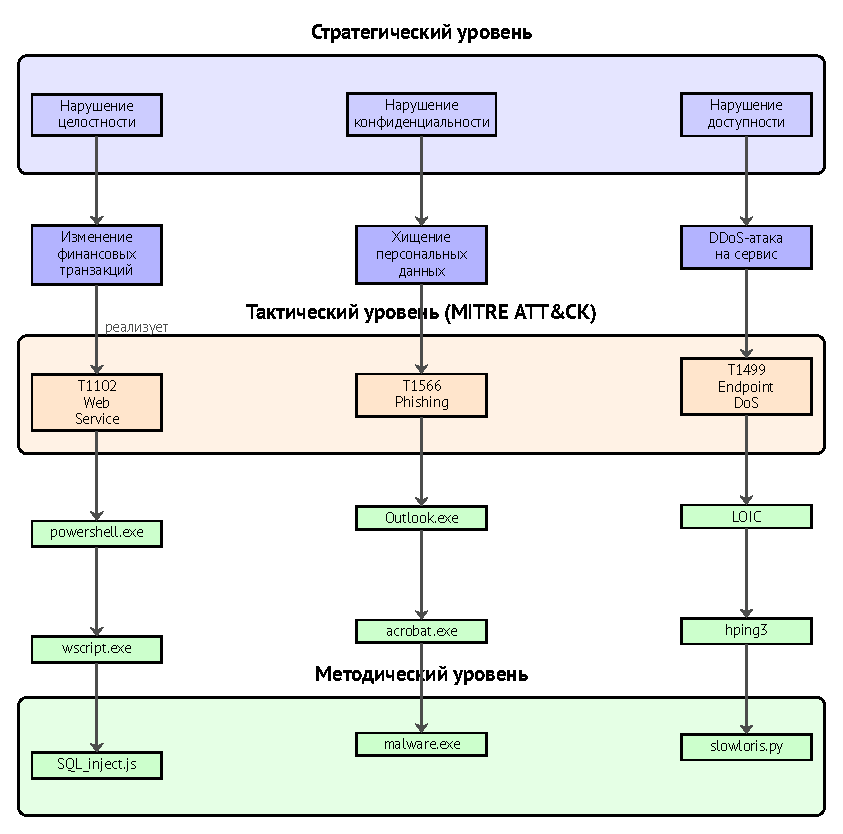
\includegraphics[width=0.85\textwidth]{images/fig_multilevel_metagraph}
\caption{Многоуровневая атрибутивная метаграфовая модель}
\label{fig:multilevel}
\end{figure}

    \item Разработана методика выявления атак, включающая архитектуру системы AMGD (Рис.~\ref{fig:siem}), алгоритм сопоставления эталонных и динамических метаграфов, а также механизм оценки риска компрометации на~основе взвешенных путей и вероятностей реализации. Предложенный алгоритм учитывает семантическое сходство атрибутов и временные окна, что повышает точность обнаружения. 
    
        % Рисунок 2: Многоуровневая модель
        \begin{figure}[ht]
        \centering
        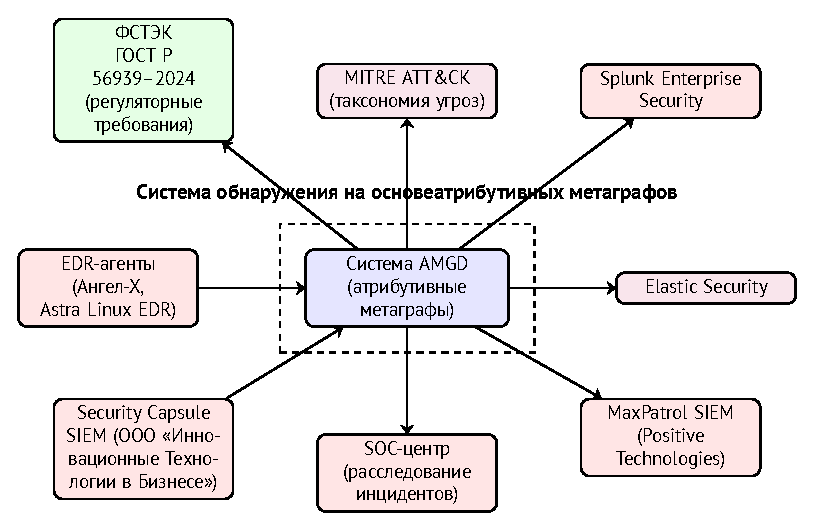
\includegraphics[width=0.85\textwidth]{images/fig_siem_integration}
        \caption{Интеграция с SIEM/SOAR}
        \label{fig:siem}
        \end{figure}

    \item Реализован прототип программной системы и проведено имитационное моделирование на данных реальных APT-кампаний (TAO, Unit 8200) и~финансово мотивированных группировок (FIN7). Экспериментальная оценка, описанная в~\cite{inside2026} и дополненная в~\cite{Latypov2025}, показала, что предложенный подход обеспечивает F1-score = 0.86, что на 22\%~выше, чем у лучших базовых методов (Таблица~\ref{tab:results}), при уровне ложных срабатываний 1.3\%.

    \item Подтверждена практическая применимость методики в пилотном проекте SOC-центра ПАО «Транснефть», где за три месяца тестирования система выявила 12 инцидентов, пропущенных стандартными правилами корреляции. Результаты согласуются с~данными, представленными в~\cite{Latypov2025}, где отмечено снижение ложных срабатываний на 19–23\%.
\end{enumerate}

Разработанная методика может быть рекомендована к~внедрению в~SIEM/SOAR-платформы (Splunk, Elastic Security, QRadar) в~качестве модуля контекстного обогащения. Она также подходит для сертификации в~соответствии с~требованиями ФСТЭК России и~ГОСТ~Р~56939–2024, поскольку обеспечивает интерпретируемость алертов и~связь технических артефактов с~бизнес-последствиями.

Перспективы дальнейшей разработки включают:
\begin{itemize}
    \item интеграцию с~фреймворком MITRE D3FEND для автоматической генерации рекомендаций по реагированию;
    \item поддержку онтологий STIX~2.1/TAXII для совместимости с~платформами обмена угрозами;
    \item внедрение механизмов самообучения на~основе больших языковых моделей (LLM) для полуавтоматического расширения библиотеки эталонных паттернов.
\end{itemize}

\pdfbookmark{Литература}{bibliography}                                % Закладка pdf
При использовании пакета \verb!biblatex! список публикаций автора по теме
диссертации формируется в разделе <<\publications>>\ файла
\verb!common/characteristic.tex!  при помощи команды \verb!\nocite!

\ifdefmacro{\microtypesetup}{\microtypesetup{protrusion=false}}{} % не рекомендуется применять пакет микротипографики к автоматически генерируемому списку литературы
\urlstyle{rm}                               % ссылки URL обычным шрифтом
\ifnumequal{\value{bibliosel}}{0}{% Встроенная реализация с загрузкой файла через движок bibtex8
    \renewcommand{\bibname}{\large \bibtitleauthor}
    \nocite{*}
    \insertbiblioauthor           % Подключаем Bib-базы
    %\insertbiblioexternal   % !!! bibtex не умеет работать с несколькими библиографиями !!!
}{% Реализация пакетом biblatex через движок biber
    % Цитирования.
    %  * Порядок перечисления определяет порядок в библиографии (только внутри подраздела, если `\insertbiblioauthorgrouped`).
    %  * Если не соблюдать порядок "как для \printbibliography", нумерация в `\insertbiblioauthor` будет кривой.
    %  * Если цитировать каждый источник отдельной командой --- найти некоторые ошибки будет проще.
    %
    %% authorvak
    \nocite{vakbib1}%
    \nocite{vakbib2}%
    \nocite{vakbib3}%
    \nocite{vakbib4}%
    \nocite{vakbib5}%
    \nocite{vakbib6}%
    \nocite{vakbib7}%
    \nocite{vakbib8}%
    \nocite{vakbib9}%
    \nocite{vakbib10}%
    \nocite{vakbib11}%
    \nocite{vakbib12}%
    %
    %% authorwos
    \nocite{wosbib1}%
    %
    %% authorscopus
    \nocite{scbib1}%
    %
    %% authorpatent
    \nocite{patbib1}%
    %
    %% authorprogram
    \nocite{progbib1}%
    %
    %% authorconf
    \nocite{confbib1}%
    \nocite{confbib2}%
    %
    %% authorother
    \nocite{bib1}%
    \nocite{bib2}%
    
    \ifnumgreater{\value{usefootcite}}{0}{
        \begin{refcontext}[labelprefix={}]
            \ifnum \value{bibgrouped}>0
                \insertbiblioauthorgrouped    % Вывод всех работ автора, сгруппированных по источникам
            \else
                \insertbiblioauthor      % Вывод всех работ автора
            \fi
        \end{refcontext}
    }{
        \ifnum \totvalue{citeexternal}>0
            \begin{refcontext}[labelprefix=A]
                \ifnum \value{bibgrouped}>0
                    \insertbiblioauthorgrouped    % Вывод всех работ автора, сгруппированных по источникам
                \else
                    \insertbiblioauthor      % Вывод всех работ автора
                \fi
            \end{refcontext}
        \else
            \ifnum \value{bibgrouped}>0
                \insertbiblioauthorgrouped    % Вывод всех работ автора, сгруппированных по источникам
            \else
                \insertbiblioauthor      % Вывод всех работ автора
            \fi
        \fi
        %  \insertbiblioauthorimportant  % Вывод наиболее значимых работ автора (определяется в файле characteristic во второй section)
        \begin{refcontext}[labelprefix={}]
            \insertbiblioexternal            % Вывод списка литературы, на которую ссылались в тексте автореферата
        \end{refcontext}
        % Невидимый библиографический список для подсчёта количества внешних публикаций
        % Используется, чтобы убрать приставку "А" у работ автора, если в автореферате нет
        % цитирований внешних источников.
        \printbibliography[heading=nobibheading, section=0, env=countexternal, keyword=biblioexternal, resetnumbers=true]%
    }
}
\ifdefmacro{\microtypesetup}{\microtypesetup{protrusion=true}}{}
\urlstyle{tt}                               % возвращаем установки шрифта ссылок URL
\end{comment}